% Monografia-LaTeX (Unochapecó)                                           %
% Copyright (C) 2013  Daniel Girotto                                      %
%                                                                         %
% This program is free software: you can redistribute it and/or modify    %
% it under the terms of the GNU General Public License as published by    %
% the Free Software Foundation, either version 3 of the License, or       %
% (at your option) any later version.                                     %
%                                                                         %
% This program is distributed in the hope that it will be useful,         %
% but WITHOUT ANY WARRANTY; without even the implied warranty of          %
% MERCHANTABILITY or FITNESS FOR A PARTICULAR PURPOSE.  See the           %
% GNU General Public License for more details.                            %
%                                                                         %
% You should have received a copy of the GNU General Public License       %
% along with this program.  If not, see <http://www.gnu.org/licenses/>.   %

% ------------------------------------------------------------ %
% Monografia                                                   %
% ------------------------------------------------------------ %
\documentclass[pnumromarab, normaltoc, a4paper, 12pt]{abnt}

% Usar \label e \ref
% \label
% \ref

\usepackage{url}
\usepackage{leading}
\usepackage{lmodern}
\usepackage{graphicx}
\usepackage{abnt-unochapeco}
\usepackage[abnt-emphasize=bf]{abnt-alf}
\usepackage{varwidth}
\usepackage{times}
\usepackage[utf8]{inputenc}
\usepackage[brazil]{babel}
\usepackage{listings}
\usepackage{listings-ext}
\usepackage{listingsutf8}

\begin{document}

\newcommand{\area}{área de ciências exatas e ambientais}
\newcommand{\curso}{ciência da computação}
\newcommand{\grau}{bacharelado}
\newcommand{\grautitulo}{bacharel}
\newcommand{\supervisortcc}{Prof. Sandro Silva de Oliveira, Me.}
\newcommand{\coordenador}{Profa. Viviane Duarte Bonfim, Ma.}
\newcommand{\membrobancaa}{Prof. Marcos Antonio Moretto, Esp.}
\newcommand{\membrobancab}{Prof. Jean Carlos Hennrichs, Esp.}
\newcommand{\datadefesa}{25 de Junho de 2013}
\newcommand{\textofolhaaprovacao}{Este trabalho de conclusão de curso foi
   julgado adequado para obtenção de título de graduação em \datadefesa, e foi
   aprovado pelo curso de \grau\  em \curso\ da \instituicao}

\renewcommand{\autor}{Andrei Jiácomo Zuse}
\renewcommand{\instituicao}{Universidade Comunitária da Região de Chapecó}
\newcommand{\instituicaosimples}{Unochapecó}
\renewcommand{\titulo}{Aplicativo Móvel para o Sistema Acadêmico Minha Uno}
\renewcommand{\local}{Chapecó}
\renewcommand{\data}{Junho de 2013}
\renewcommand{\comentario}{Relatório do Trabalho de Conclusão de Curso submetido
  à Universidade \mbox{Comunitária} da Região de Chapecó para obtenção do título
  de bacharel em Ciência da Computação.}
\renewcommand{\orientador}{Prof. Marcelo Cezar Pinto, Me.}

\capa
\folhaderosto
\folhadeaprovacao


% \resumo {Conteúdo do resumo} {Palavras-Chave}
\resumo{Este trabalho apresenta um aplicativo para dispositivos móveis para o sistema acadêmico Minha Uno, permitindo que os acadêmicos da universidade acessem por meio de um aplicativo as informações da sua graduação. Utilizando-se de técnicas de extração de dados a partir do código HTML da página do sistema acadêmico Minha Uno e implementando um servidor REST, posteriormente consumido pela aplicação. Desta forma o trabalho divide-se em duas linhas práticas, abordando o servidor de extração de informações do sistema acadêmico, e outra onde é exibida a implementação da aplicação, consumindo as informações do servidor implementado e mostrando ao usuário em seu dispositivo com o sistema operacional Google Android ou iOS. Os módulos implementados foram escolhidos por meio de questionário online aplicado aos acadêmicos, assim como as plataformas a serem contempladas com a aplicação e outras informações sobre o perfil dos acadêmicos que utilizam o Sistema Acadêmico Minha Uno. Ao final do trabalho é possível concluir que o servidor implementado pode fornecer informações não apenas para o aplicativo móvel, mas também para outros aplicativos que venham a ser desenvolvidos, e que a implementação de um aplicativo para dispositivos móveis é de desejo da comunidade acadêmica e é viável a sua implementação.}
{Aplicativo Móvel; Extração de Informações; Sistema Acadêmico; Unochapecó}

% \abstract {Abstract content} {Keywords}
\abstract{This paper presents a mobile application for the academic system Minha Uno, allowing university academics to access through an application the information of their graduation. Using techniques of data extraction from the HTML page of the academic system Minha Uno and implementing a REST server subsequently consumed by the application. Thus the work is divided into two practices lines, one addressing the de data extraction server from academic system, and another which opens the implementation of the application, consuming the  information server implemented and showing the user on your device with the operating system Google Android or iOS. The modules implemented were chosen through online questionnaire applied to academics, as well as the platforms to be included with the application and other information about the profile of the students who use the Academic System Minha Uno. At the end of the study it can be concluded that the implemented server can provide information not only for the mobile application, but also for other applications that may be developed, and that the implementation of an application for mobile devices is the desire of the academic community and is feasible implementation.}
{Mobility; Server; Extraction; Communication; Unochapecó}

\addcontentsline{toc}{chapter}{LISTA DE FIGURAS}
\listoffigures

\addcontentsline{toc}{chapter}{LISTA DE TABELAS}
\listoftables

% ------------------------------------------------------------ %
% Altera o título do Sumário                                   %
% ------------------------------------------------------------ %
\renewcommand{\contentsname}%
  {\vspace*{.8cm}
  \normalsize{\bfseries\MakeUppercase{sumário}}%
  \vspace{1.4cm}}

\sumario

\chapter{Introdução}

A adoção de dispositivos móveis com sistema operacional Android e iOS chegam a níveis nunca antes vistos na história da tecnologia. Comparada com outras tecnologias recentes, a adoção de dispositivos do tipo smart foi dez vezes mais rápida que a revolução dos Computadores Pessoais nos anos 80, duas vezes mais rápida que a explosão da Internet nos anos 90 e três vezes mais rápida que a adoção de Redes Sociais. Estima-se que, no mundo, existam 640 milhões de dispositivos com iOS e Android em uso durante o mês de Julho de 2012
\cite{flurry2012}.

No período de Julho de 2011 a Julho de 2012, o Brasil apresentou o 3º maior crescimento no número de dispositivos móveis, com um aumento de 220\%. Estima-se que o Brasil possua 13 milhões de dispositivos com iOS e Android ativos, ocupando o décimo lugar no ranking mundial de dispositivos móveis ativos
\cite{flurry2012}.

Em dados da Huawei (fabricante dos equipamentos utilizados pelas operadoras de telefonia móvel) em seu balanço anual, no Brasil houve um aumento de 99\% no número de usuários da tecnologia 3G. Até o mês de Abril do ano de 2012, em relação ao final de 2011, ocorreu um aumento de 31\% no número de usuários e levando-se em consideração o intervalo do primeiro trimestre de 2011 até o primeiro trimestre de 2012, houve um aumento de 112,6\% no número de usuários
\cite{Huawei1T2012}.

Considerando válida a suposição de que a expansão e uso de dispositivos móveis e tecnologia 3G é similar ao do Brasil na região de Chapecó, pode-se verificar pelos números do balanço social 2011 da Fundação Universitária do Desenvolvimento do Oeste (FUNDESTE), instituição mantenedora da Universidade Comunitária da Região de Chapecó (Unochapecó), que o número de pessoas vinculadas a universidade com acesso a estas tecnologias é significativo. Segundo o balanço social 2011, a Unochapecó conta com 947 funcionários sendo destes 540 docentes e 407 técnico-administrativos. Segundo este mesmo documento, a instituição conta com 8031 acadêmicos de graduação e 910 acadêmicos de pós-graduação, totalizando 8941 acadêmicos ao final do ano de 2011 \cite{Fundeste2011}. Atualmente todas estas pessoas, acadêmicos ou funcionários da Universidade utilizam uma página web para acessar as informações do(s) seu(s) perfil(s), chamada “Minha Uno''. Deste universo de quase 9 mil pessoas, pode-se estimar com base nos dados anteriormente vistos que mais de 600 pessoas envolvidas com a universidade possuam smartphones ou tablets.

\section{Tema}
Devido a crescente utilização de dispositivos móveis (tablets e smartphones) no meio acadêmico, e a facilidade de acesso a internet sem fio e móvel, pretende-se com este trabalho melhorar o acesso ao sistema acadêmico da Universidade Comunitária da Região de Chapecó (Unochapecó) nos mesmos, por meio do desenvolvimento de um aplicativo que notifique o usuário sobre novas informações no sistema e também permita a consulta aos dados do sistema conforme suas permissões, além de poder efetuar cadastros.

\section{Delimitação do Problema}
Tendo como ponto de partida o funcionamento atual do Sistema Acadêmico (Minha Uno), existe uma forma de melhorar a forma de acesso em dispositivos móveis por meio de um aplicativo, agregando recursos que auxiliem os usuários do mesmo?

\section{Questões de Pesquisa}
Quais funcionalidades do sistema acadêmico os usuários desejam que esteja presente em seus dispositivos móveis? 

Qual tecnologia de desenvolvimento multiplataforma para dispositivos móveis se adapta melhor as necessidades de desenvolvimento da aplicação? 

Qual será a forma de comunicação com o sistema acadêmico atual, para a coleta das informações necessárias para o funcionamento nos dispositivos móveis?

Quais as plataformas que serão contempladas com esta aplicação? 

Como permitir que o usuário acesse as informações sem estar conectado a internet?
\section{Objetivos}
\subsection{Objetivo Geral}
Melhorar a forma de acesso ao Sistema Acadêmico em dispositivos móveis por meio de um aplicativo para consulta das informações pertencentes ao perfil do usuário, além de notificações sobre alterações no sistema que sejam de interesse do utilizador da aplicação.

\subsection{Objetivos Específicos}
Definir por meio de um questionário aplicado aos usuários do Sistema Acadêmico quais funcionalidades são importantes para cada perfil de usuário existente no sistema, e posteriormente definir quais destas funcionalidade estarão disponíveis no aplicativo.

Planejar para que a aplicação a ser desenvolvida e sua implantação cause o menor impacto possível na infraestrutura atual da instituição.

Pesquisar qual tecnologia de desenvolvimento multiplataforma fornece os recursos necessários para o desenvolvimento da aplicação.

Definir juntamente com a equipe de Tecnologia da Informação da instituição a forma de comunicação com o Sistema Acadêmico, assim como quais informações serão disponibilizadas pela instituição. 

Por meio do questionário efetuado com os usuários do Sistema Acadêmico, levantar as plataformas móveis mais utilizadas para desenvolver a aplicação.

Definir quais eventos ocorridos no Sistema Acadêmico são importantes, para assim notificar os usuários sobre os mesmos. 
\section{Justificativa}

A utilização de dispositivos móveis vem batendo records de crescimento a cada ano, superando outras inovações tecnológicas consideradas fundamentais nos dias de hoje, como os Computadores Pessoais, a Internet e as Redes Sociais, estimando-se que existam 640 milhões de dispositivos móveis com sistema operacional Android ou iOS sendo utilizados no mundo durante o mês de Julho de 2012. O Brasil apresentou o terceiro maior crescimento na adoção deste tipo de dispositivos entre 2011 e 2012, tendo um crescimento de 220\% no número de usuários, ficando atrás da China com aumento de 401\% e do Chile com aumento de 279\% neste mesmo período. Além disto, o Brasil encontra-se em décimo lugar no ranking de dispositivos móveis com Sistema Operacional Android ou iOS, com 13 milhões de dispositivos ativos, atrás dos Estados Unidos com 165 milhões de dispositivos, China com 128 milhões, Reino Unido com 31 milhões, Coréia do Sul com 28 milhões de dispositivos, Japão com 22 milhões de dispositivos, Alemanha com 19 milhões de dispositivos, França com 17 milhões de dispositivos, Canadá com 16 milhões de dispositivos e Espanha com 13 milhões de dispositivos
\cite{flurry2012}.

Também percebe-se aumento de 26,2\% na utilização de internet banda larga 3G no mundo no período de 2010 até 2011. No Brasil houve um aumento mais significativo, chegando a 99\% no mesmo período, passando de 20,6 milhões de usuários em 2010 para 41,1 milhões de usuários em 2011. Tendo como período para avaliação desde o primeiro trimestre de 2011 até o primeiro trimestre de 2012, percebe-se um aumento de 112,6\% no número de usuários de conexão banda larga 3G no país \cite{Huawei1T2012}.

Apesar do grande aumento no número de usuários destas tecnologias, o país ainda não se encontra saturado de dispositivos móveis, como ocorre, por exemplo, em Singapura, onde 92\% das pessoas entre 15 e 64 anos possuem um dispositivo móvel com Android ou iOS, tendo assim um crescimento anual discreto no número de usuários devido a esta saturação. Nos Estados Unidos o número de pessoas entre 15 e 64 anos que possuem este tipo de dispositivo totalizam 310 milhões de pessoas, 78\% da população esta faixa etária \cite{flurry2012}.

Em uma pesquisa semelhante feita por acadêmicos da Universidade de Minho (localizada em Braga, Portugal) durante o ano de 2008, constatou-se que entre as 1225 pessoas de diferentes centros de ensino superior de Portugal que participaram da pesquisa, apenas 1\% das pessoas pesquisadas não possuem dispositivos móveis (\emph{Personal Digital Assitant} (PDA), smartphones). Levando-se em consideração o crescimento das plataformas móveis nos anos posteriores a este período, com o lançamento da primeira geração do iPhone no ano de 2008 em Portugal, e posteriormente a popularização da plataforma Android nos anos subsequentes, mostra que o uso de Celulares, smartphones, PDA's (e atualmente tablets) é popular nos meios acadêmicos deste país \cite{UsoTecnologiasMoveisEstudantesPortugueses}. Devido a Portugal ser um país desenvolvido e o Brasil ser um país em desenvolvimento, esta pesquisa pode não refletir a quantidade real da utilização nas instituições de ensino superior no Brasil ou da Unochapecó, mas demonstra que a utilização de dispositivos móveis em meios acadêmicos é comum, ficando até mesmo acima da média nacional. 

Por meio de uma pesquisa semelhante a realizada em Portugal, sendo esta aplicada na Unochapecó durante o desenvolvimento deste trabalho, será possível definir o percentual de usuários dentre os pesquisados que utilizam dispositivos móveis para acesso ao sistema acadêmico, e também definir quais as funcionalidades do Sistema Acadêmico Minha Uno são mais importantes para os usuários de cada perfil, podendo assim servir como base para o desenvolvimento da aplicação, atendendo diretamente as necessidades dos usuários do mesmo.

Tendo como ponto de partida a escolha das funcionalidades do sistema, é necessário definir as ferramentas utilizadas na implementação do aplicativo. Para isto, deve-se avaliar as três categorias de ferramentas de desenvolvimento para mobilidade multiplataforma existentes (Compilação Cruzada, Máquina Virtual e Webkit) para definir qual melhor atente das necessidades no desenvolvimento da aplicação. Cada classe de ferramentas possui um propósito, possuindo pontos positivos e negativos a serem levados em consideração durante o desenvolvimento da aplicação \cite{CrossPlatformMobileDevelopment2011}.

Para efetuar-se a integração entre aplicativos para dispositivos móveis e páginas web, são disponibilizados web services, que utilizando de protocolos como o \emph{Simple Object Access Protocol} (SOAP), \emph{Web Services Description Language} (WSDL), \emph{Universal Description Discovery and Integration} (UDDI) (ou outras tecnologias mais recentes como o \emph{JavaScript Object Notation} (JSON)), disponibilizam informações via Linguagem Extensível de Marcação (XML) para outras aplicações \cite{WebApplicationArchitecture}.  Tem-se como exemplo disto o Facebook, que disponibiliza uma \emph{Application programming interface} (API) de desenvolvimento, que extrai informações dos webservices, e também permite inserção de novas informações utilizando-se destas mesmas ferramentas \cite{Facebook}.




\section{Procedimentos Metodológicos}

Esta pesquisa ocorre de forma quantitativa, aplicando um questionário defindo para obter as informações relevantes ao desenvolvimento do projeto e implementação. Os métodos utilizados para a elaboração deste projeto serão feitos através de pesquisa bibliográfica, artigos retirados da internet, coleta de dados feita através de questionário e desenvolvimento de um protótipo de acesso ao sistema para dispositivos móveis.

Quanto à coleta de dados, será feito um questionário com alunos, professores e funcionários da Unochapecó, para levantar informações sobre os usuários do Sistema Acadêmico Minha Uno.  Após o término do questionário e interpretação dos dados coletados, serão determinadas quais as funcionalidades do sistema acadêmico são mais relevantes para seus usuários, percentual de usuários que possuem smartphones, tablets ou ambos, os sistemas operacionais móveis mais utilizados pelos mesmos e a principal forma de acesso a internet utilizada em seus dispositivos móveis. A partir destes dados será possível determinar quais as prioridades no desenvolvimento da aplicação e a divisão das etapas de desenvolvimento da mesma, tendo em vista nas etapas iniciais as funcionalidades mais importantes para cada perfil de usuário.

A pesquisa bibliográfica no aspecto de desenvolvimento para dispositivos móveis e integração com webservice, conta com um número considerável de obras e autores. Portanto, este trabalho acadêmico, neste ponto, terá suas necessidades supridas.



\section{Desenvolvimento}
\chapter{Revisão Bibliográfica}

\section{Tecnologias}

\subsection{Sistema Operacional para Dispositivos Móveis}
Sistemas operacionais para dispositivos móveis seguem o mesmo conceito aplicado a outras plataformas, que segundo Tanembaum, é de difícil definição por meio de um único conceito, pois o mesmo é responsável pelo Gerenciamento do Hardware hospedeiro do mesmo, como também fornecer um conjunto de recursos abstratos claros em vez de recursos confusos de hardware aos aplicativos \cite{tanenbaum2010modern}. Em outras palavras, pode-se dizer que o sistema operacional é formado de um conjunto de softwares e bibliotecas que tornam mais fácil a interação entre a máquina e os usuários.

\subsubsection{Symbian}
Desenvolvido pela parceria entre Nokia, Ericsson, Motorola e PSION, foi usado amplamente pela Nokia em praticamente todos os seus dispositivos no passado. O sistema operacional tinha como foco a integridade e segurança de dados, evitar desperdício de tempo do usuário e trabalhar com recursos escassos. Era reconhecido pelo gerenciamento extremamente eficiente de recursos como bateria, processador e memória\cite{SistemasOperacionaisMoveisComputacao}.

\subsubsection{iOS}
Desenvolvido pela Apple, tendo como base o sistema operacional Mac OS X, o iOS inicialmente foi desenvolvido para iPhone, depois expandido para outros produtos como iPad e iPod. É o único sistema operacional analisado desenvolvido para dispositivos específicos, sendo totalmente fechado aos mesmos. Apresenta um ótimo desempenho devido a integração entre Hardware e Software, além da interface gráfica intuitiva, porém apresenta dificuldades para interagir com outros dispositivos externos (como por exemplo outros celulares utilizando a tecnologia Bluetooth) \cite{AvaliacaoComparativaSOMoveis}.

\emph{\bf{MELHORAR DESCRIÇAO iOS}}

\subsubsection{Google Android}
O Google Android surgiu da necessidades de várias empresas fabricantes de Hardware, Software e Operadoras de Telefonia Móvel de um sistema operacional que apresentasse vantagens para os desenvolvedores de Software e uma experiência de usuário inovadora, com muitos recursos sem abrir mão da beleza e da facilidade de uso. Desenvolvido pela Open Handset Alliance \cite{OHA}, o Google Android é um sistema operacional desenvolvido sobre o kernel Linux com aplicações nativas e a possibilidade desenvolvimento de aplicações por qualquer pessoa que possua as habilidades e vontade para isso \cite{lechetagoogle}.

\emph{\bf{MELHORAR DESCRIÇAO GOOGLE ANDROID}}

\subsubsection{Windows Phone}
Lançado pela Microsoft em 2010, como sucessor do Windows Mobile, o Windows Phone foi desenvolvido para atender tanto usuários comuns como corporativos. O Windows Phone foi desenvolvido para rodar em diversos hardwares, podendo ser licenciado pelas fabricantes que desejarem usar o mesmo em seus dispositivos. Possui integração total com o ambiente .NET também da Microsoft, além das tecnologias de desenvolvimento Silverlight e XNA. Apresenta uma desvantagem em relação aos outros sistemas operacionais que é não possuir multithread, permitindo que apenas uma aplicação seja executada por vez no dispositivo \cite{AvaliacaoComparativaSOMoveis}.

\subsection{Web service}
Web service é um sistema de software que permite a comunicação entre diversos softwares por meio de mensagens SOAP, normalmente utilizando o Protocolo de transferência de Hipertexto (HTTP) para transmitir arquivos de dados entre as aplicações \cite{W3C}.
\subsubsection{REST}
A arquitetura de Transferência de Estado Representativo (do inglês \emph{Representational State Transfer}, também identificado como REST) é uma técnica da engenharia de software que define uma interface uniforme de conexão. O REST é um estilo híbrido, baseado em muitos protocolos baseados em rede (como Protocolo Cliente-Servidor, Protocolo de Sistemas em Camadas, Protocolo de Sessão Remota, etc.) \cite{RESTFielding}.



%\url{http://www.ics.uci.edu/~fielding/pubs/dissertation/rest_arch_style.htm}

\section{JavaScript}
\url{https://developer.mozilla.org/en-US/docs/Web/JavaScript?redirectlocale=en-US&redirectslug=JavaScript}
\subsection{JSON}
\url{http://www.json.org/json-pt.html}

\section{Java}
\url{http://www.java.com/pt_BR/download/whatis_java.jsp}

\section{SQLite}
\url{http://www.sqlite.org/}

\section{Jsoup}
\url{https://github.com/jhy/jsoup/blob/master/README}
\\ \url{http://jsoup.org/}

\section{Ferramentas de Desenvolvimento Multiplataforma para Dispositivos Móveis}
Um dos grandes desafios para os desenvolvedores de software é encontrar qual ferramenta atende as necessidades da aplicação a ser desenvolvida. Isso fica ainda mais perceptível quando a aplicação deve ser executada em dispositivos móveis, devido a diversidade de sistemas operacionais a serem atendidos. Hoje existem 4 sistemas operacionais para dispositivos móveis que detém grande parte do mercado, sendo eles Android, iOS, Windows Phone e Symbian, sendo o Android e o iOS detentores da maior fatia do mercado. Ao se deparar com este cenário, desenvolvedores se perguntam qual tipo de ferramenta permite que eles desenvolvam apenas uma vez a aplicação, e que a mesma rode de forma satisfatória em todos os dispositivos. Abaixo será visto as 3 principais técnicas de desenvolvimento multiplataforma para dispositivos móveis\cite{CrossPlatformMobileDevelopment2011}.

\subsection{Compilação Cruzada}
Ferramentas do tipo Compilação Cruzada separam os ambientes de compilação conforme a plataforma de destino, gerando código fonte nativo para a plataforma de destino neste momento do processo de geração de um aplicativo. Com isso são geradas aplicações que são nativas para as plataformas alvo. Este tipo de ferramenta possui a desvantagem de consumir mais tempo durante a compilação, devido a conversão de código, e por apresentar certa demora para aderir a novas plataformas
\cite{CrossPlatformMobileDevelopment2011}.

\subsubsection{Titanium}
Desenvolvido pela Appcelerator, o Titanium foi lançado em dezembro de 2008. Baseado na técnica de compilação cruzada, o desenvolvedor utiliza-se de uma API JavaScript para o desenvolvimento da aplicação, e no momento da compilação são gerados códigos nativos para a diferentes plataformas. A compilação é composta por 3 etapas, sendo elas: Pré compilação (Otimização do código JavaScript), Compilação de Front-End (Geração de código nativo da plataforma alvo) e Compilação e Empacotamento para a plataforma (Geração do aplicativo). A diferença entre o Titanium e os outros frameworks descritos abaixo é a geração de interfaces que não utilizam de um motor de navegação, mas que são nativas, geradas por código nativo resultante da compilação do código JavaScript
\cite{CrossPlatformMobileDevelopment2011}.

Devido a estas características nativas, que torna difícil e demorado o suporte a novas plataformas, o Titanium suporta no formato de compilação cruzada apenas os sistemas operacionais iOS e Android, além de suportar desenvolvimento baseado em Web utilizando HTML5
\cite{appceleratorTitanium}.

\subsection{Máquina Virtual}
Ferramentas do tipo Máquina Virtual ficam entre as ferramentas baseadas em Web e as ferramentas de Compilação Cruzada. Nelas o código-fonte é empacotado juntamente com bibliotecas e uma máquina virtual, que em tempo de execução converte os comandos do código fonte em comandos nativos da plataforma que está executando a aplicação. Sua desvantagem é que normalmente aplicações maiores apresentam um certo delay na sua execução, devido a conversão do código
\cite{CrossPlatformMobileDevelopment2011}.

\subsubsection{Rhodes}
Lançado em 2008, o Rhodes é um framework para desenvolvimento que faz parte do ecossistema de ferramentas voltadas para o desenvolvimento multiplataforma. Por se utilizar de uma Máquina virtual para a execução dos programas desenvolvidos, o mesmo converte as aplicações desenvolvidas utilizando Ruby na sua parte lógica, e \emph{HyperText Markup Language} (HTML), JavaScript e \emph{Cascading Style Sheets} (CSS) para a interface gráfica para código nativo da plataforma em que a aplicação está sendo executada, apresentando uma experiência de usuário similar a de aplicações desenvolvidas em código nativo para a plataforma em que a aplicação está sendo executada
\cite{CrossPlatformMobileDevelopment2011}.

\subsection{Web}
Ferramentas do tipo Web empacotam código fonte voltado para a internet (normalmente desenvolvidos em HTML e CSS) juntamente com um Webkit, dando a impressão para o usuário que se trata de uma aplicação desenvolvida para aquela plataforma. Possui como principal vantagem o desenvolvimento simplificado porém , por não utilizar componentes gráficos do sistema operacional hospedeiro, apenas simula o comportamento de uma aplicação nativa. Além disso, depende dos recursos fornecidos pelo webkit do sistema operacional para determinar o nível de acesso a funcionalidades do mesmo 
\cite{CrossPlatformMobileDevelopment2011}.

\subsubsection{PhoneGap}
Criado no inicio de 2008, o PhoneGap fornece um conjunto de ferramentas para desenvolvimento de aplicações multiplataforma para dispositivos móveis utilizando apenas código HTML, JavaScript e CSS. Muito popular pela sua flexibilidade, arquitetura simples e de fácil utilização. Utilizando um modelo híbrido de execução, um único código-fonte escrito em HTML, JavaScript e CSS são executados em um browser empacotado em forma de aplicação nativa, suportado em cada plataforma de destino. O Acesso as funcionalidades do Sistema Operacional é feito por meio da chamada de métodos JavaScript que fazem as requisições na API proprietária do Sistema Operacional. É uma alternativa para a portabilidade de aplicações Web para dispositivos móveis, mas deve-se lembrar que não se possui acesso aos componentes gráficos nativos do sistema operacional
\cite{CrossPlatformMobileDevelopment2011}.

\section{Comunicação}

\subsection{Redes Sem Fio}
As redes sem fio tem como principal característica não haver necessidade de cabos para conectar vários dispositivos. Este tipo de rede apresenta uma complexidade maior comparada com as redes cabeadas, devido a mobilidade dos dispositivos, o que não ocorre com os dispositivos utilizados nas redes com fio, onde a mobilidade máxima é a permitida pelo cabo ao qual o dispositivo está conectado. Além disso, neste tipo de rede podem ocorrer problemas de interferência entre redes que compartilham o mesmo espaço físico 
\cite{IEEE80211}.

\emph{\bf{MELHORAR DESCRIÇAO REDES WIFI}}

\subsection{Telefonia e Internet Móvel}
Desde a primeira geração de telefones móveis introduzidas no mundo durante os anos 80 e 90  até a atual tecnologia 4G (LTE) muitas evoluções ocorreram na forma como os celulares se comunicam. A evolução causada por estas tecnologias mudou a forma em que o mundo se comunica, trazendo a possibilidade de conectar-se a internet utilizando um dispositivo móvel onde quer que você esteja, bastando haver sinal da operadora de telefonia.

\subsubsection{1G}
As redes de 1ª Geração (1G) causaram grande impacto na sociedade pelo seu nível de inovação. Trabalhando de forma analógica utilizando-se de modulação de frequência (do inglês Frequency Modulation - FM), onde se transmitia a voz do usuário em faixas de Frequência Muito Alta (do inglês Ultra High Frequency - UHF) \cite{AEvolucaoTelefoniaCelular}. Este tipo de rede permite apenas o tráfego de voz, onde a qualidade das ligações varia conforme o nível de interferência. Além disso um dos problemas desta tecnologia é a baixa segurança, onde é possível fazer escuta de ligações utilizando-se de sintonizador de rádio e até mesmo utilizar frequências alheias para efetuar ligações  \cite{GeracoesTelefoniaMovel}.

\subsubsection{2G}
Inserida no mercado no início da década de 90, é marcada pela mudança da tecnologia analógica para a tecnologia digital, permitindo assim além de um maior número de ligações simultâneas na rede, o envio de mensagens de texto (\emph{Short Message Service} (SMS)) e a capacidade de transmitir dados em baixa velocidade entre dispositivos utilizando-se da rede \cite{GeracoesTelefoniaMovel}.

\subsubsection{3G}
A terceira geração de redes móveis é considerada um avanço nas redes 2G baseadas na família de normas da União Internacional de Telecomunicações. Trouxe as redes maior capacidade e serviços para os usuários, como conexões de dados a longas distancias com velocidades variando entre 5 e 10Mbps \cite{GeracoesTelefoniaMovel}.

\subsubsection{4G}
Absorvendo todas as características das redes 3G, as redes 4G propõe mais velocidade e uma nova visão de mercado. Este padrão totalmente baseado em endereçamento IP garante velocidades de acesso entre 100Mbps com dispositivos em movimento e 5Gbps para dispositivos em repouso. Como o 4G é totalmente baseado em IP, também torna possível a integração de qualquer dispositivo que utilize desta tecnologia, como web TV's, gadgets. A tecnologia prevê a serviços como envio de Mensagens Multimídia (do inglês \emph{Multimedia Messaging Service} - MMS), Video Chat, TV Móvel, Broadcast de Video Digital além dos serviços básicos como voz e dados. Além disso prevê a a interoperabilidade entre os diversos padrões de rede sem fio \cite{GeracoesTelefoniaMovel}.

\chapter{Sistema Acadêmico Minha Uno}

Desenvolvido pela Unochapecó, o sistema acadêmico “Minha Uno'' é a interface utilizada pelos acadêmicos, docentes e funcionários da universidade para envio e recebimento de informações.

O sistema consiste em uma página web, dividida em perfis, com opções diferentes para cada um deles. O sistema é composto pelos perfis “Graduação'', “Pós-Graduação'', “Professor'', “Técnico-Administrativo'', “Administrador'', “Fornecedor'' e “Apoio-Operacional''.

Dentre os perfis existentes no sistema, foram avaliados os perfis: Professor, Graduação, Pós-Graduação e Técnico-Administrativo.


\section{Graduação}
O perfil de graduação é voltado aos acadêmicos dos diferentes cursos da Unochapecó. Por meio dele, 
os acadêmicos são informados das  suas notas, recebem novos materiais, 
se informam da sua situação financeira, solicitam documentos entre outras opções.

Com uma interface confusa em alguns momentos, porém de modo geral de fácil aprendizado, 
a mesma é de uso obrigatório para qualquer graduando da instituição, pois sem ela não é possível 
acompanhar as notas, entregar alguns trabalhos ou tirar os boletos para o pagamento das mensalidades. 
Abaixo lista completa das opções fornecidas por este perfil: \\
- Atividades Curriculares Complementares \\
- Bolsa de Estudo \\
- Bolsa de Pesquisa \\
- Cadastro de Objetos Pedidos \\
- Componentes Curriculares Fora da Matriz \\
- Componentes Curriculares Isolados \\
- Componentes Curriculares Turno Diferenciado \\
- Conhecimento Prévio \\
- Disponibilidade de Laboratórios de Informática \\
- Dúvidas/Sugestões \\
- E-mail \\
- Entrega de Trabalhos \\
- Ficha de Matrícula \\
- Financiamento \\
- Formulário para Negociação Diferenciada \\
- Histórico \\
- Horários de Aula/Ementas/Requisitos \\
- Horários do Semestre \\
- Inscrições em Eventos \\
- Inscrições para Estágio \\
- Material de Apoio/Planos de Ensino \\
- Negociação pela Internet \\
- Notas Graduação \\
- Pedidos de Livros Livraria Universitária \\
- Programa de Incentivos \\
- Protocolo Digital \\
- Quero Livro - Curso de Direito \\
- Renovação de Matricula \\
- Situação Financeira \\
- Solicitação de Documentos \\
- Solicitação de Estágio - Cursos de Direito e Farmácia \\
- Titulos a Receber e \\
- Trancamento parcial. \\

O layout do sistema acadêmico e a disposição dos itens pode ser visualizado na Figura 1.

\begin{figure}[!htb]
     \centering
     \caption[Layout do Sistema - Perfil Graduação]{Layout do perfil Graduação do Sistema Acadêmico Minha Uno.}
     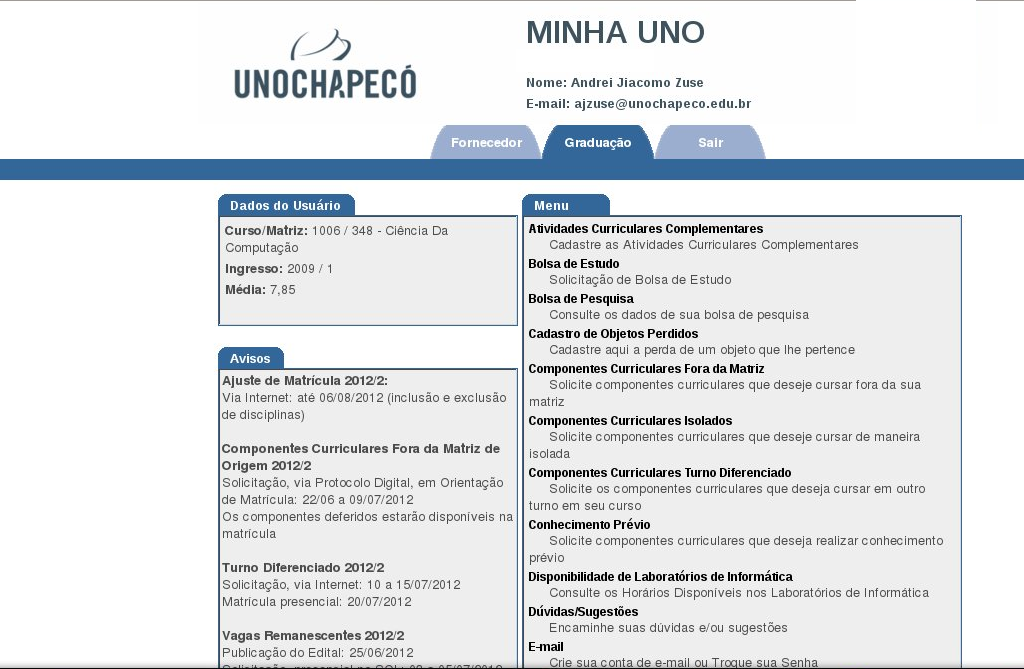
\includegraphics[scale=0.3]{imagens/GraduacaoCorrigida.png}
     \\ Fonte: Do Autor
\end{figure}

\newpage
\section{Pós-Graduação}
O perfil de pós-graduação é voltado aos acadêmicos dos diferentes cursos de pós-graduação da Unochapecó. 
Por meio dele, os acadêmicos são informados das  suas notas, recebem novos materiais, 
se informam da sua situação financeira, solicitam documentos entre outras opções.

Com uma interface mais limpa que a apresentada pelo perfil de graduação, a mesma é de uso obrigatório para qualquer 
pós-graduando da instituição, pois sem ela não é possível acompanhar as notas, entregar alguns trabalhos ou 
tirar os boletos para o pagamento das mensalidades. As opções presentes neste perfil são: \\
- Cadastro de Objetos Perdidos \\
- Dúvidas/Sugestões \\
- E-mail \\
- Ementas \\
- Entrega de Trabalhos \\
- Inscrições em Eventos \\
- Material de Apoio/Planosd e Ensino \\
- Notas Pós-Graduação \\
- Pedidos de Livros Livraria Universitária \\
- Programa de Incentivos \\
- Protocolo Digital \\
- Situação Financeira \\
- Solicitação de Documentos e \\
- Títulos a Receber. \\

O layout do sistema acadêmico e a disposição dos itens pode ser visualizado na Figura 2.

\begin{figure}[!htb]
     \centering
     \caption[Layout do Sistema - Perfil Pós-Graduação]{Layout do perfil Pós-Graduação do Sistema Acadêmico Minha Uno.}
     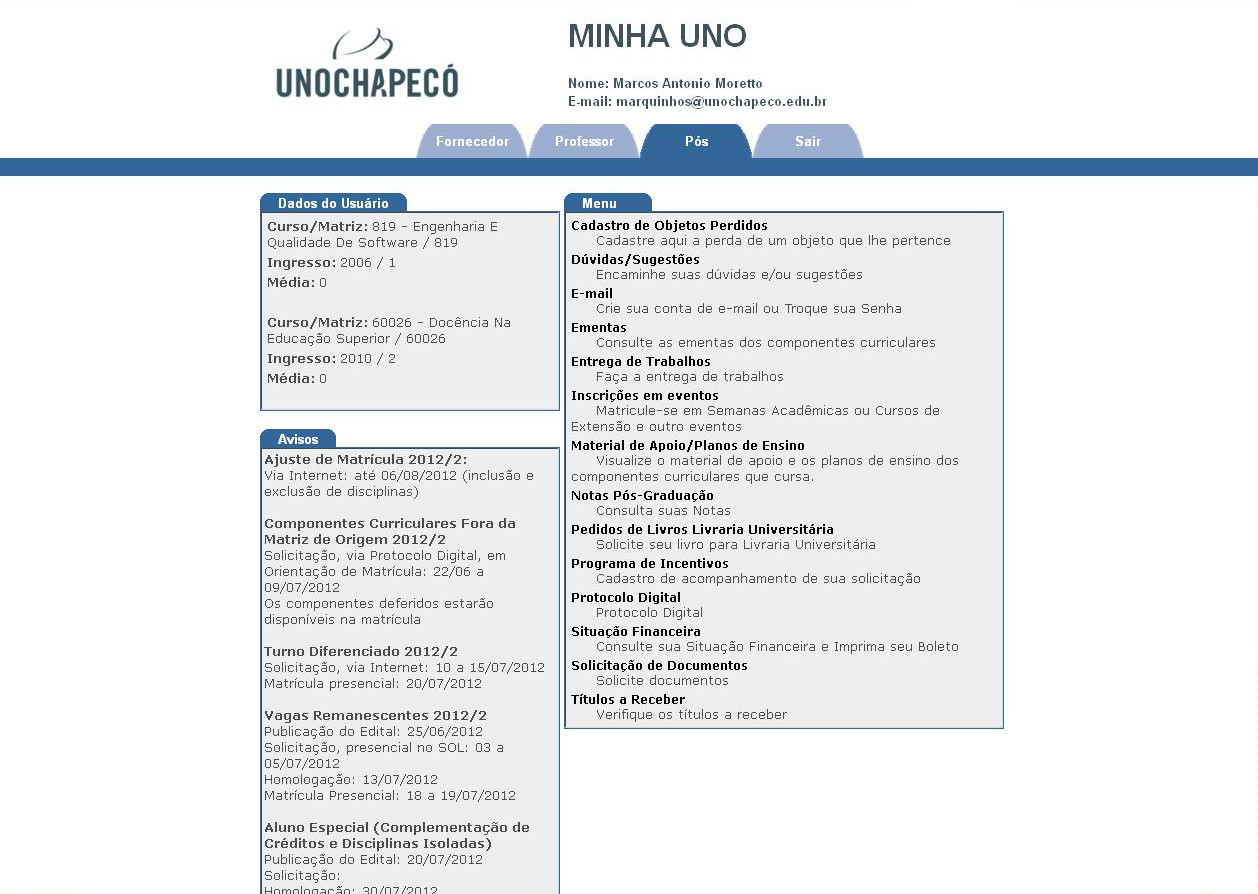
\includegraphics[scale=0.3]{imagens/pos.jpg}
     \\ Fonte: Do Autor
\end{figure}

\section{Professor}
Utilizado pelos docentes da instituição, o perfil de Professor pode ser considerado o painel de controle das disciplinas
ministradas. Utilizando-se do perfil no Sistema Acadêmico o professor coloca novos materiais nas disciplinas ministradas,
adiciona as notas dos alunos, envia mensagens aos mesmos, efetua as chamadas entre outras funcionalidades.
As opções disponíveis neste perfil são: \\
- Cadastro de Objetos Perdidos \\
- Cadastro de Veículo \\
- Componentes Curriculares Complementares \\
- Comunicação Interna Eletrônica \\
- Contato RH \\
- Diário de Classe On-Line \\
- Documentos Diversos \\
- E-mail \\
- Entrega de Trabalhos \\
- Envio de Projetos de Pesquisa \\
- Folha de Pagamento \\
- Gastos dos Convênios Asser \\
- Horários de Aula/Ementas/Requisitos \\
- Horários do Professor \\
- Inscrições em Eventos \\
- Ligações Telefônicas \\
- Material de Apoio \\
- Pedidos de Livros Livraria Universitária \\
- Período de Férias \\
- Plano de Ensino \\
- Plano Mensal de Trabalho do Professor \\
- Processo Seletivo \\
- Programa de Aprendizagem \\
- Quero Livro - Curso de Direito \\
- Ramais \\
- Registro das Atividades Mensais \\
- Relatório on-line/Projetos de pesquisa \\
- Repositório de Arquivos \\
- Reservas \\
- Reservas Laboratório de Informática \\
- Sistema de Mensagem Integrada \\
- Solicitação de Coffee Break e \\
- Sumula de Currículo. \\

O layout do sistema acadêmico e a disposição dos itens pode ser visualizado na Figura 3.


\begin{figure}[!htb]
     \centering
     \caption[Layout do Sistema - Perfil Professor]{Layout do perfil Professor do Sistema Acadêmico Minha Uno.}
     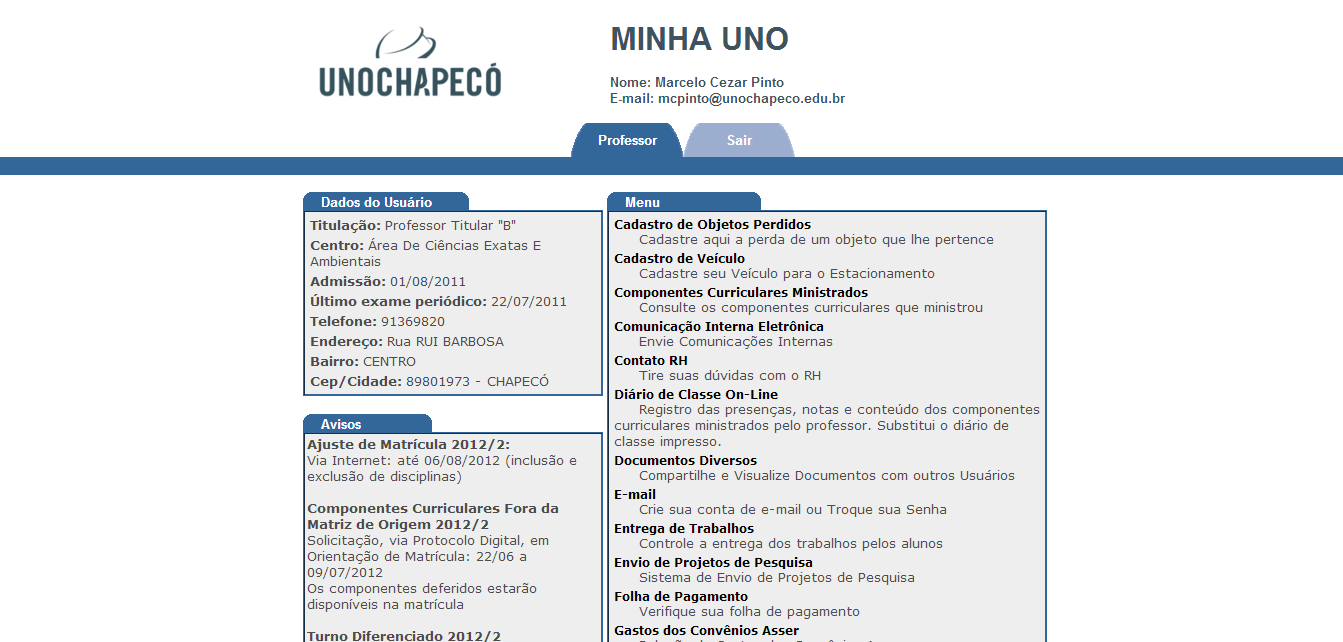
\includegraphics[scale=0.4]{imagens/professor.png}
     \\ Fonte: Do Autor
\end{figure}

\newpage

\section{Técnico-Administrativo}
Utilizado pelos Funcionários da Unochapecó para comunicação interna, entrar em contato com o setor de Recursos Humanos (RH),
consultar sua folha de pagamento, participar de processos seletivos entre outras tarefas, o perfil Técnico-Administrativo
possui as seguintes opções: \\
- Cadastro de Artigos/Monografias/TCC \\
- Cadastro de Objetos Perdidos \\
- Cadastro de Veículo \\
- Cartão-Ponto \\
- Comunicação Interna Eletrônica \\
- Contato RH \\
- Documentos Diversos \\
- E-mail \\
- Folha de Pagamento \\
- Gastos dos Convênios Asser \\
- Inscrições em Eventos \\
- Ligações Telefônicas \\
- Pedidos de Livros Livraria Universitária
- Período de Férias \\
- Processo Seletivo \\
- Ramais \\
- Repositório de Arquivos \\
- Reservas \\
- Reservas Laboratório de Informática \\
- Sistema de Mensagem Integrada \\
- Solicitação de Coffee Break \\
- Sumula de Currículo e \\
- Títulos a Receber. \\

O layout do sistema acadêmico e a disposição dos itens pode ser visualizado na Figura 1.


\begin{figure}[!htb]
     \centering
     \caption[Layout do Sistema - Perfil Técnico-Administrativo]{Layout do perfil Técnico-Administrativo do Sistema Acadêmico Minha Uno.}
     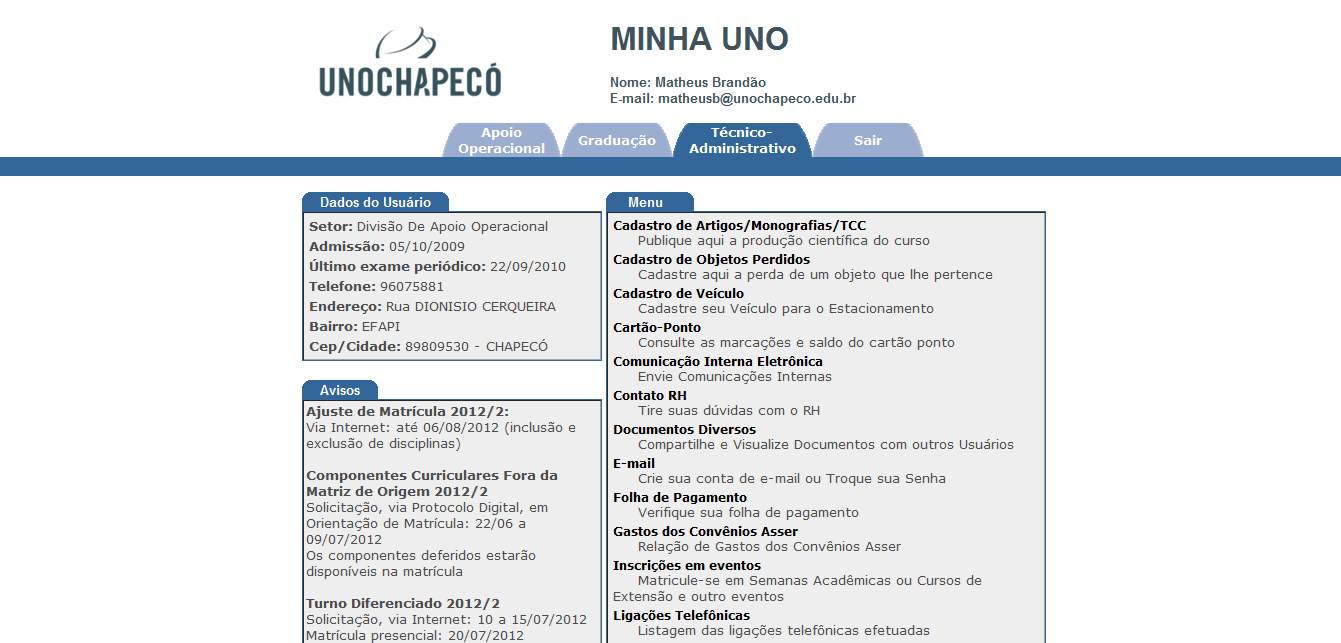
\includegraphics[scale=0.4]{imagens/tecnico.png}
     \\ Fonte: Do Autor
\end{figure}
\chapter{Questionário}
Com a finalidade de obter informações sobre a utilização de dispositivos móveis no meio acadêmico, e descobrir a importância de cada item presente no sistema acadêmico atual, entre os dias 25 de agosto de 2012 e 26 de setembro do mesmo ano foi realizado questionário virtual com o corpo acadêmico da universidade. 

Ao total 281 pessoas responderam o questionário, sendo obtidas 300 respostas sobre os diferentes perfis do sistema acadêmico. O questionário teve sua estrutura dividida em três partes, sendo a primeira sobre a utilização de smartphones e tablets no meio acadêmico, a segunda parte sobre a relevância de cada item presente no sistema acadêmico atual (Minha Uno) e a terceira parte sobre o interesse de participar dos testes do aplicativo.

Para o questionário, o perfil “Técnico-Administrativo'' foi tratado como “Funcionários'', sendo esta a nomenclatura adotada na avaliação dos dados coletados. 

\section{Utilização de Dispositivos Móveis}
A primeira parte do questionário foi aplicada específicamente para pessoas que possuem dispositivos móveis do tipo smartphone ou tablet (ou ambos), totalizando 126 pessoas (44,84\% dos entrevistados). 

Com o objetivo de descobrir quais os sistemas operacionais dos dispostivos móveis dos participantes do questionário, foi feita a seguinte pergunta: “Qual o sistema operacional do seu smartphone ou tablet'', sendo as alternativas “Android'', “iOS'', “Windows Phone'', “Symbian'', “Outros'', “Não Sei'' e que foi permitido ao usuário marcar mais de uma alternativa. Os resultados obtidos com esta pergunta mostraram que 56,25\% dos participantes utilizam aparelhos com o sistema operacional Android, seguidos por 17,97\% com iOS, 10,16\% com Symbian, 3,91\% com Windows Phone e 1,56\% com Outros Sistemas Operacionais. Pessoas que não sabiam qual o sistema operacional do seu smartphone ou tablet totalizaram 10,16\%.

Com o objetivo de descobrir qual a forma de acesso a internet móvel mais comum entre os participantes do questionário, foi feita a eles a pergunta “Você utiliza o dispositivo móvel para acessar a internet?'' com as opções “Sim, 3G e Wi-fi'', “Sim, Apenas 3G'', “Sim, Apenas Wi-fi'' e “Não'', sendo que o participante poderia selecionar apenas uma das opções. Obteve-se que 46,83\% dos usuários acessam apenas internet Wi-fi dos seus dispositivos. Em segundo lugar, temos os usuários que acessam internet 3G e Wi-fi, com 45,24\% das respostas. Em terceiro lugar aparecem os usuários que não acessam a internet pelos seus dispositivos móveis, com 4,76\% e em quarto lugar os usuários que acessam a internet apenas via 3G, com 3,17\%.

A última questão feita nesta etapa do questionário se referia ao fato de acessar o sistema acadêmico dos seus dispostivos móveis, sendo que 50,79\% dos participantes informaram que não constuma acessar o sistema acadêmico dos seus dispositivos móveis enquanto o restante (49,21\%) efetuam este tipo de acesso. 

A partir dos dados analisados acima, é possível verificar que, a partir do percentual de participantes que possuem dispositivos móveis, e com os dados do balanço social de 2011 da Fundeste (instituição mantentenedora da Unochapecó), considerando apenas o percentual de pessoas que acessam o sistema acadêmico pelos dispositivos móveis atualmente, aproximadamente 2181 pessoas seriam beneficiadas diretamente com o desenvolvimento de uma aplicação para dispositivos móveis, sendo que se considerar o percentual total de usuários de smartphones ou tablets entrevistados, este número sobe para 4434 pessoas beneficiadas.

\section{Relevância de cada item presente no sistema acadêmico atual}
Com o objetivo de descobrir quais opções disponíveis atualmente no sistema acadêmico são relevantes para os usuários, esta parte do questionário foi dividida em quatro subpartes, onde perguntas específicas sobre cada perfil de acesso do sistema acadêmico foram criadas. 

Ao entrar nesta sessão de perguntas, o usuário inicialmente selecionou qual perfil do sistema acadêmico ele faz parte, e posteriormente foi redirecionado as perguntas específicas de cada perfil. Ao fim das perguntas, o mesmo foi direcionado novamente para o formulário de seleção de perfis, para caso possua acesso a mais de um perfil de usuário, poder responder as perguntas referentes aos outros perfis.

Os perfis de interesse do questionário são os perfis referentes aos alunos de Graduação, alunos de Pós-Graduação, Professores e Funcionários, não constando no questionário o perfil Fornecedor ou outros perfis do sistema acadêmico.

Participaram desta etapa do questionário 281 usuários, onde o perfil “Graduação'' obteve 280 respostas, o perfil “Pós-Graduação'' obteve uma resposta, o perfil “Professor'' obteve duas respostas e o perfil “Funcionário'' obteve 17 respostas.

\subsection{Graduação}

Esta parte do questionário foi destinada apenas para estudantes de cursos de Graduação, onde o acadêmico deu notas de 1 a 5 para cada item disponível no sistema acadêmico atual, utilizando-se da escala de Likert, onde  a nota 1 demonstra que o item menos importante para o acadêmico, e a nota 5 representa que o item é importantíssimo.

Na tabela 1 serão representadas as perguntas efetuadas e a média final das respostas. Esta parte da pesquisa contou com 280 respostas, 93,33\% do total de respostas da pesquisa.
\begin{table}[!hbt]
\centering
\caption[Média de Respostas dos Alunos de Graduação]{Média de Respostas dos Alunos de Graduação sobre os itens do sistema acadêmico}
\vspace{3mm}
\begin{tabular}{p{9.5cm}|c}\hline
\textbf{Item} & \textbf{Média Final} \\ \hline
Bolsa de Pesquisa & 2,84 \\ \hline
Disponibilidade de Laboratório de Informática & 2,46 \\ \hline
Entrega de Trabalhos & 3,70 \\ \hline
Histórico & 3,79 \\ \hline
Horário de Aula/Ementas/Requisitos & 4,29 \\ \hline
Horários do Semestre & 4,39 \\ \hline
Material de Apoio/Planos de Ensino & 4,80 \\ \hline
Notas da Graduação & 4,53 \\ \hline
Situação Financeira & 4,24 \\ \hline
\textbf{Média} & \textbf{3,8} \\ \hline
\textbf{Desvio-Padrão} & \textbf{0,79} \\ \hline
\end{tabular}
\\ Fonte: elaboração do autor.
\end{table}

Aplicando-se a distribuição t de Student, representada pela fórmula 
\[
t=\frac{{\overline{X}} - \mu_0}
{\frac{S_c}{\sqrt{n}}}
\]
onde:\\ 
- $\overline{X}$ é a média amostral observada; \\
- $\mu_0$ é a média esperada, sendo esta 3 na pesquisa; \\
- $S_c$ o desvio padrão amostral corrigido, e; \\
- $n$ é o tamanho da amostra analisada.

O desvio-padrão amostral corrigido é calculado por meio da fórmula 
\[
   S_c = \sqrt{\frac{1}{n-1} \sum_{i=1}^n(X_i - \overline{X})^2} 
\]
Que apresenta parâmetros semelhantes aos utilizados na fórmula utilizada no cálculo da distri- \\ buição t de Student, com o acréscimo do $X_i$ que representa o valor observado para o indivíduo $i$ da amostra
\cite{DistroStudent}.

Aplicando-se as fórmulas acima a tabela 1, foram obtidos os valores apresentados na tabela 2.

\begin{table}[!hbt]
\centering
\caption[Avaliação dos dados obtidos - Graduação]{Avaliação dos dados obtidos com as respostas dos alunos de graduação}
\vspace{3mm}
\begin{tabular}{p{5cm}|c|c|c|c}\hline
\textbf{Item} & \textbf{Média} & \textbf{$S_c$} & \textbf{$t$} & \textbf{Índice de Confiança (\%)} \\ \hline
Bolsa de Pesquisa & 2,84 & 1,435 & -1,9158 & 94,35 \\ \hline
Disponibilidade de Laboratório de Informática & 2,46 & 1,351 & -6,6773 & 99,99 \\ \hline
Entrega de Trabalhos & 3,70 & 1,350 & 8,7214 & 99,99 \\ \hline
Histórico & 3,79 & 1,272 & 10,339 & 99,99 \\ \hline
Horário de Aula/Ementas/Requisitos & 4,29 & 1,067 & 20,221 & 99,99  \\ \hline
Horários do Semestre & 4,39 & 0,906 & 25,738 & 99,99 \\ \hline
Material de Apoio/Planos de Ensino & 4,80 & 0,553 & 54,334 & 99,99 \\ \hline
Notas da Graduação & 4,53 & 0,552 & 46,475 & 99,99 \\ \hline
Situação Financeira & 4,24 & 0,903 & 22,899 & 99,99 \\ \hline
\end{tabular}
\\ Fonte: elaboração do autor.
\end{table}

O cálculo do índice de confiança pode ser reproduzido utilizando-se da função INVT (ou similar) do editor de planilhas eletrônicas, sendo que os percentuais apresentados no índice de confiança foram arredondados para duas casas decimais para permitir melhor interpretação do mesmos. 
Devido a utilização da  distribuição t de Student na forma bicaudal, nos casos onde o valor $t$ apresentou-se negativo, o índice de confiança representa o percentual de chances de a resposta ficar abaixo da média em pesquisas feitas posteriormente, enquanto em itens onde o valor $t$ apresentou-se positivo, o percentual de confiança demonstra as chances de em pesquisas posteriores os valores ficarem acima da média.

\subsection{Pós-Graduação}
Esta parte do questionário foi destinada apenas para estudantes de cursos de Pós-Graduação, onde o pós-graduando deu notas de 1 a 5 para cada item disponível no sistema acadêmico atual, utilizando-se da escala de Likert, onde  a nota 1 demonstra que o item menos importante para o acadêmico, e a nota 5 representa que o item é importantíssimo.

Na tabela 3 serão representadas as perguntas efetuadas e a média final das respostas. Esta parte da pesquisa contou com 1 resposta, não sendo assim possível extrair informações conclusivas sobre este perfil do sistema acadêmico.

\begin{table}[!hbt]
\centering
\caption[Média de Respostas dos Alunos de Pós-Graduação]{Média de Respostas dos Alunos de Pós-Graduação sobre os itens do sistema acadêmico}
\vspace{3mm}
\begin{tabular}{p{9.5cm}|c}\hline
\textbf{Item} & \textbf{Média Final} \\ \hline
Ementas & 3,00 \\ \hline
Entrega de Trabalhos & 5,00 \\ \hline
Material de Apoio/Planos de Ensino & 5,00 \\ \hline
Notas da Pós-Graduação & 5,00 \\ \hline
Situação Financeira & 5,00 \\ \hline
\textbf{Média} & \textbf{4,60} \\ \hline
\textbf{Desvio-Padrão} & \textbf{0,89} \\ \hline
\end{tabular}
\\ Fonte: elaboração do autor.
\end{table}

Devido a possuir apenas uma resposta, não foi efetuada avaliação de Student sobre este item para medir o índice de confiança da resposta obtida, pois o tamanho da amostra pode ser considerada insignificante para a tomada de decisões.

\subsection{Professor}
Esta parte do questionário foi destinada apenas para o corpo docente da instituição onde o professor deu notas de 1 a 5 para cada item disponível no sistema acadêmico atual, utilizando-se da escala de Likert, onde  a nota 1 demonstra que o item menos importante para o acadêmico, e a nota 5 representa que o item é importantíssimo.

Na tabela 4 serão representadas as perguntas efetuadas e a média final das respostas. Esta parte da pesquisa contou com 2 respostas, não sendo assim possível extrair informações conclusivas sobre este perfil do sistema acadêmico.

\begin{table}[!hbt]
\centering
\caption[Média de Respostas dos Professores]{Média de Respostas dos Professores sobre os itens do sistema acadêmico}
\vspace{3mm}
\begin{tabular}{p{9.5cm}|c}\hline
\textbf{Item} & \textbf{Média Final} \\ \hline
Componentes Curriculares Ministrados & 1,50 \\ \hline
Diário de Classe Online & 5,00 \\ \hline
Documentos Diversos & 1,00 \\ \hline
Entrega de Trabalhos & 4,50 \\ \hline
Folha de Pagamento & 2,00 \\ \hline
Gastos dos Convênios Asser & 1,50 \\ \hline
Horários de Aula/Ementas/Requisitos & 4,50 \\ \hline
Horários do Professor & 4,00 \\ \hline
Ligações Telefônicas & 2,00 \\ \hline
Material de Apoio & 5,00 \\ \hline
Período de Férias & 1,00 \\ \hline
Plano de Ensino & 4,00 \\ \hline
Processo Seletivo & 2,00 \\ \hline
Programa de Aprendizagem & 3,00 \\ \hline
Ramais & 3,00 \\ \hline
Registro de Atividades Mensais & 2,50 \\ \hline
Sistema de Mensagens Integrada & 4,00 \\ \hline
\textbf{Média} & \textbf{2,97} \\ \hline
\textbf{Desvio-Padrão} & \textbf{1,40} \\ \hline
\end{tabular}
\\ Fonte: elaboração do autor.
\end{table}

\newpage

Além das questões referentes aos itens acima, também foi feita a pergunta \emph{Sobre o item “Diário de Classe Online'', seria interessante a possibilidade de fazer chamadas e registrar notas pelo smartphone ou tablet?} sendo que 100\% dos participantes responderam afirmativamente.

Devido a possuir apenas duas respostas, não foi efetuada avaliação de Student sobre este item para medir o índice de confiança das respostas obtidas, pois o tamanho da amostra pode ser considerada insignificante para a tomada de decisões.

%\newpage

\subsection{Funcionário}
Esta parte do questionário foi destinada apenas para os funcionários da instituição onde o funcionário deu notas de 1 a 5 para cada item disponível no sistema acadêmico atual, utilizando-se da escala de Likert, onde  a nota 1 demonstra que o item menos importante para o acadêmico, e a nota 5 representa que o item é importantíssimo.

Na tabela 5 serão representadas as perguntas efetuadas e a média final das respostas. Esta parte da pesquisa contou com 17 respostas.

\begin{table}[!hbt]
\centering
\caption[Média de Respostas dos Funcionários]{Média de Respostas dos Funcionários sobre os itens do sistema acadêmico}
\vspace{3mm}
\begin{tabular}{p{9.5cm}|c}\hline
\textbf{Item} & \textbf{Média Final} \\ \hline
Cartão-Ponto & 4,29 \\ \hline
Folha de Pagamento & 4,59 \\ \hline
Gastos dos Convênios Asser & 2,24 \\ \hline
Ligações Telefônicas & 3,00 \\ \hline
Período de Férias & 3,41 \\ \hline
Processo Seletivo & 3,35 \\ \hline
Ramais & 3,65 \\ \hline
Sistema de Mensagem Integrada & 3,59 \\ \hline
Súmula de Currículo & 3,12 \\ \hline
Títulos a Receber & 3,41 \\ \hline
\textbf{Média} & \textbf{3,46} \\ \hline
\textbf{Desvio-Padrão} & \textbf{0,66} \\ \hline
\end{tabular}
\\ Fonte: elaboração do autor.
\end{table}

Aplicando-se a distribuição t de Student, explicada na seção 7.2.1, foram obtidos os índices de confiança mostrados na tabela 6.

\begin{table}[!hbt]
\centering
\caption[Avaliação dos dados obtidos - Funcionário]{Avaliação dos dados obtidos com as respostas dos funcionários da instituição}
\vspace{3mm}
\begin{tabular}{p{5cm}|c|c|c|c}\hline
\textbf{Item} & \textbf{Média} & \textbf{$S_c$} & \textbf{$t$} & \textbf{Índice de Confiança (\%)} \\ \hline
Cartão-Ponto & 4,29 & 0,314 & 16,986 & 99,99 \\ \hline
Folha de Pagamento & 4,59 & 0,190 & 34,388 & 99,99 \\ \hline
Gastos dos Convênios Asser & 2,24 & 0,344 & -9,4499 & 99,99 \\ \hline
Ligações Telefônicas & 3,00 & 0,339 & 0 & 0 \\ \hline
Período de Férias & 3,41 & 0,306 & 5,5489 & 99,99 \\ \hline
Processo Seletivo & 3,35 & 0,293 & 4,9738 & 99,98 \\ \hline
Ramais & 3,65 & 0,359 & 7,4393 & 99,99 \\ \hline
Sistema de Mensagem Integrada & 3,59 & 0,306 & 7,927 & 99,99\\ \hline
Súmula de Currículo & 3,12 & 0,292 & 1,662 & 88,5 \\ \hline
Títulos a Receber & 3,41 & 0,282 & 6,0298 & 99,99 \\ \hline
\end{tabular}
\\ Fonte: elaboração do autor.
\end{table}

O item “Ligações Telefônicas'' apresentou indice de confiança igual a 0 pois a média obtida no mesmo é igual a média esperada ($\mu_0$) para o questionário, tornando a parte superior da fórmula apresentada na seção 7.2.1 zero. Sendo assim a média a ser obtida em questionários posteriores pode ser superior ou inferior a obtida neste questionário.

Para os outros itens aplicam-se as regras presentes na seção 7.2.1, o cálculo do índice de confiança pode ser reproduzido utilizando-se de um editor de planilhas eletrônicas, sendo que neste trabalho os percentuais apresentados no índice de confiança foram arredondados para duas casas decimais para permitir melhor interpretação do mesmos. 

Devido a utilização da  distribuição t de Student na forma bicaudal, nos casos onde o valor $t$ apresentou-se negativo, o indice de confiança representa o percentual de chances de a resposta ficar abaixo da média em pesquisas feitas posteriormente, enquanto em itens onde o valor $t$ apresentou-se positivo, o percentual de confiança demonstra as chances de em pesquisas posteriores os valores ficarem acima da média.

\section{Avaliação dos dados coletados}
Avaliando-se os resultados obtidos no questionário, dados estes apresentados anteriormente, observa-se que os perfis utilizados pelos professores e alunos de pós-graduação não possuem informações suficientes para se chegar a conclusões sobre os itens importantes ou não do sistema.
Por outro lado, os perfis utilizados pelos funcionários e estudantes de graduação obtiveram uma quantidade maior de respostas, fornecendo assim dados mais conclusivos sobre a relevancia dos itens presentes nestes perfis.

Conclui-se que para a implementação do aplicativo para dispositivos móveis, deve-se observar os itens que obtiveram maior relevância nestes perfis em que foi possível efetuar uma análise mais detalhada, onde os itens que obtiveram maiores médias terão maior prioridade sobre os itens que obtiveram médias menores. Além disso, os itens que ficaram com suas médias abaixo de 3,00 não serão considerados importantes na etapa inicial de desenvolvimento, sendo implementados apenas caso haja tempo suficiente após os itens com maiores médias serem implementados no aplicativo.

\section{Interesse em participar dos testes da nova aplicação}
Contando apenas com duas perguntas, a etapa final do questionário teve como objetivos levantar interessados em auxiliar nos testes da aplicação, e obter o contato das pessoas interessadas. Tendo como base os pesquisados que possuem smartphone ou tablet, 99,21\% demonstraram interesse em auxiliar nos testes da nova aplicação.

\section{Implementação}
Com base nos dados apresentados neste capítulo, optou-se em serem implementado apenas o perfil dos alunos de graduação, devido ao número de respostas trazer informações mais confiáveis sobre as opções mais utilizadas pelos acadêmicos. Além disso, devido a forma de extração das informações ocorrer de forma manual e depender do layout da página do sistema acadêmico atual, foi optado por implementar os três módulos com melhores médias (Material de Apoio/Planos de Ension, Notas da Graduação e Horários do Semestre), para demonstrar a possibilidade da extração e também possuir informações reais para a aplicação móvel, extraidas diretamente do Sistema Acadêmico Minha Uno.

\chapter{Servidor}
Com o objetivo de extrair e preparar as informações a serem consumidas pela aplicação móvel do sistema acadêmico Minha Uno, foi desenvolvido em linguagem Java um servidor REST para facilitar e agilizar a extração dos dados. 

Como no questionário apresentado anteriormente obtemos maior quantidade de respostas referentes aos acadêmicos de cursos de graduação, então para este trabalho foi escolhido implementar o servidor e posteriormente a aplicação para este público alvo, sendo implementados os módulos que apresentaram as três melhores notas, sendo eles Material de Apoio, Notas da Graduação e Horários do Semestre.

Utilizando-se da biblioteca \emph{jsoup} para a extração das informações e após o tratamento dos dados gerando-se arquivos JSON transmitidos utilizando um servidor REST, serão detalhadas nas próximas sessões o funcionamento de cada etapa da extração, preparação e transmissão das informações desde o sistema acadêmico Minha Uno até a aplicação móvel.

\section{Ferramentas Utilizadas}
Para o desenvolvimento do servidor foram utilizadas apenas ferramentas Open-Source, sendo que a linguagem escolhida para o desenvolvimento foi o Java, devido a quantidade de documentação encontrada na internet, e também por possuir bibliotecas prontas que permitem a extração, tratamento e disponibilidade das informações, facilitando assim a implementação do servidor.

\section{Extração das Informações}

Segundo informações obtidas da diretoria de Ti da Unochapecó, a instituição não possui um webservice com as informações do sistema acadêmico, e desta forma as informações exibidas na página são extraidas diretamente de uma coleção de banco de dados, o que tornaria inviável a integração direta com estas bases. Com a excasses de alternativas, foi necessário extrair as informações diretamente da página do sistema acadêmico. Para todos os processos de extração foi utilizada a biblioteca \emph{jsoup}, sendo que a mesma é responsável pela conexão aos diferentes endereços do sistema acadêmico e pela extração das informações a partir do retorno das consultas de navegação, ou seja, sendo extraidas as informações a partir do HTML retornado pelo sistema acadêmico atual.

Após o devido tratamento utilizando-se filtros com expressão regular e outros comandos permitidos pelo \emph{jsoup}, as informações necessárias para a aplicação são obtidas, sendo que na continuidade do capítulo será explicado como cada grupo de informações foi extraido e posteriormente preparado para ser consumido pelos dispositivos móveis.

Todas as expressões utilizadas na biblioteca \emph{jsoup} podem ser testadas na página web \url{http://try.jsoup.org/} utilizando como entrada o código HTML da página a ser analizada. Mais informações sobre as expressões utilizadas podem ser obtidas em \url{http://jsoup.org/cookbook/extracting-data/selector-syntax}.

Como toda a extração é baseada no retorno do código HTML do sistema atual, qualquer alteração no layout do arquivo HTML retornado pela página do sistema acadêmico Minha Uno resultará em problemas na extração dos dados.


\subsection{Login}
Com o objetivo de validar se o login fornecido pelo usuário na aplicação é válido e extrair o cookie (identificador de sessão utilizado para as acesso as informações obtidas apenas pelo login válido do usuário), o servidor possuí como primeira tarefa ao receber uma solicitação da aplicação a validação de login.

Utilizando-se do método POST do HTTP, os dados de login são enviados utilizando o endereço \url{https://www.unochapeco.edu.br/usuarios/login?login_submited=1&usuario=USUARIO&senha=SENHA&submit=entrar} (as palavras USUARIO e SENHA devem ser substituidas pelas respectivas informações).


O algoritmo de extração do cookie e validação do login não apresenta nenhuma complexidade, conforme pode-se observar no Apendice A.1 deste trabalho.

%%% Aqui é a sessão de extração do material de apoio
\subsection{Material de Apoio}
Com o objetivo de extrair a relação dos materiais eletrônicos postados pelos professores em cada disciplina cursada pelo acadêmico. Para melhor entendimento, o algoritmo será dividido em duas partes, sendo que a primeira parte mostrará como são extraidas as informações referentes as disciplinas cursadas pelo acadêmico, e a segunda parte do como são extraidas as informações dos materiais disponíveis.

%%% Aqui é a subsubsessão de extração das disciplinas
\subsubsection{Extração das Disciplinas}
Com o objetivo de extrair a lista das disciplinas pertencentes ao módulo de material de apoio do sistema acadêmico, é necessário que a informação seja extraida a partir do código HTML retornado pela url \url{https://www.unochapeco.edu.br/saa/materialApoio.php}. Para a obtenção das disciplinas corretas cursadas pelo acadêmico, é utilizado o cookie de sessão capturado no momento do login, conforme explicado no item 5.2.1 deste trabalho. Um exemplo de código HTML retornado pelo servidor a partir deste tipo de consulta pode ser visto na url \url{http://goo.gl/fLo0h}.

A partir do código HTML retornado, sendo aplicanda a expressão ``\emph{form tr td:eq(1) a}'' sob o mesmo por meio da biblioteca \emph{jsoup}, obtém-se como retorno a lista das disciplinas cursadas pelo acadêmico, conforme pode ser visto na figura 5.

\begin{figure}[!htb]
     \centering
     \caption[Extração de Informações - Lista de Disciplinas do Material de Apoio]{Lista das disciplinas extraidas.}
     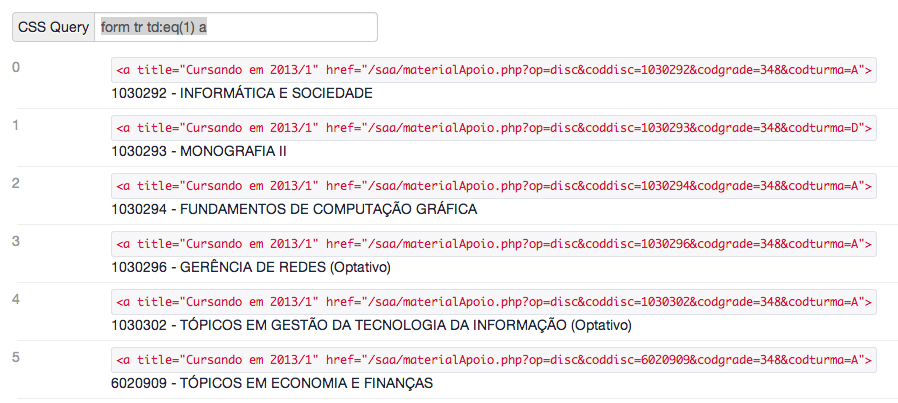
\includegraphics[scale=0.5]{imagens/listadisciplinasmaterialapoio.png}
     \\ Fonte: Do Autor.
\end{figure}

A partir da lista retornada acima, é possível retornar diretamente a disciplina no formato ``\emph{Código - Nome}''. Também como pode-se verificar na Imagem 5, acima do nome da disciplina é exibida a tag HTML completa, sendo que nesta tag pode-se verificar o atributo \emph{href}, que possui o caminho completo para serem extraidos os materiais da disciplina.

Após a extração do nome da disciplina e da tag \emph{href}, é necessária a extração das informações dos materiais da disciplina, explicada na sessão 5.2.2.2 deste trabalho.

%%% Aqui é a subsubsessão de extração dos materiais
\subsubsection{Extração dos Materiais}
Após a extração da lista de disciplinas e da referência ao endereço web onde as disciplinas podem ser acessadas, é necessário extrair as informações dos materiais propriamente ditos.

A partir do código HTML (disponível na url \url{http://goo.gl/jB8ia}, sendo que o mesmo é pertencente a uma disciplina do 9º período de Ciência da Computação na grade 348) obtido pela url capturada (conforme explicado na sessão 5.2.2.1). No código retornado, existem 4 informações relevantes, sendo elas: nome, url, publicação e descrição.

Para a extração do nome do material, a expressão ``\emph{form tr:contains(Arquivo) a}'', sendo que a mesma retorna uma lista com o nome das disciplinas, conforme pode ser visto na Figura 6.

\begin{figure}[!htb]
     \centering
     \caption[Extração de Informações - Lista de Nomes dos Materiais de uma disciplina]{Lista de nomes dos materiais de uma disciplina.}
     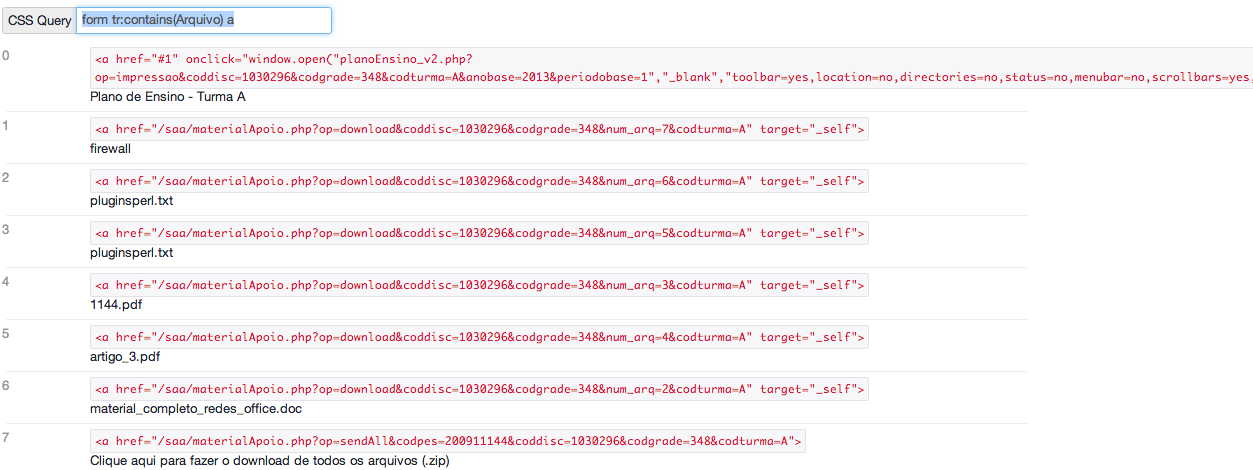
\includegraphics[scale=0.35]{imagens/listamateriaisdisciplinasnomematerial.png}
     \\  Fonte: Do Autor.
\end{figure}

Verificamos na Figura 6 que a mesma expressão retorna no campo principal o nome das disciplinas, e na sua referência (exibida em vermelho) o campo href, que nos é interessante para o acesso direto ao arquivo listado. Desta forma, utilizando-se da mesma expressão é possível extrair a url de acesso direto ao arquivo e também o nome do arquivo a ser acessado. Desta forma, duas informações já são preenchidas a partir da mesma consulta. 

Para obtermos a publicação, que nada mais é o nome do professor que postou o material e a data de postagem, utiliza-se a expressão ``\emph{form tr:contains(Publicação) td:eq(1)}'', e o seu retorno pode ser verificado na Figura 7.

\begin{figure}[!htb]
     \centering     
     \caption[Extração de Informações - Lista das publicações dos materiais]{Lista de publicação dos materiais de uma disciplina.}
     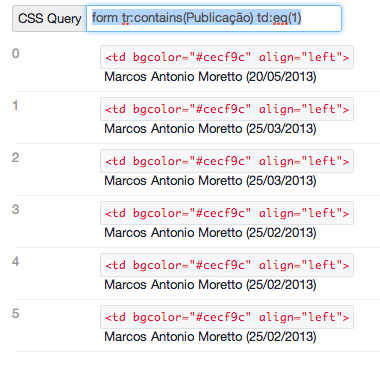
\includegraphics[scale=0.7]{imagens/listamateriaisdisciplinaspublicacao.png}
     \\  Fonte: Do Autor.
\end{figure}

Para obtermos a descrição dos materiais postados, a expressão ``\emph{form tr:contains(Descrição) td:eq(1)}'' onde obtém-se como resultado a lista da descrições dos materiais, confome pode ser visto na Figura 8.

\begin{figure}[!htb]
     \centering
     \caption[Extração de Informações - Lista das descrições dos materiais]{Lista de descrição dos materiais de uma disciplina.}
     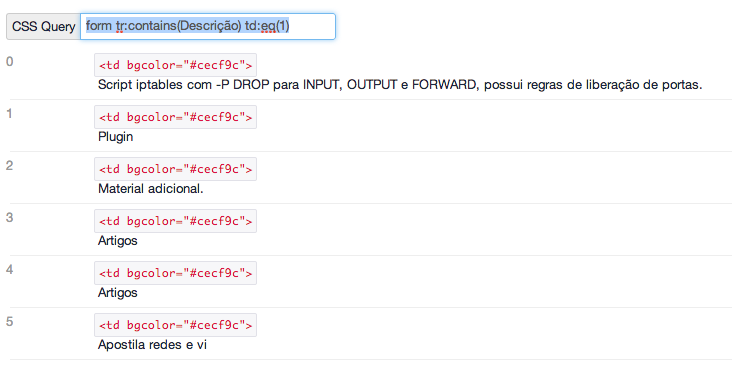
\includegraphics[scale=0.6]{imagens/listamateriaisdisciplinasdescricao.png}
     \\  Fonte: Do Autor.
\end{figure}

\subsection{Notas da Graduação}
Com o objetivo de de extrair as avaliações e as respectivas notas das avaliações aplicadas aos acadêmicos, foi desenvolvida a classe de extração das notas da graduação. Para melhor entendimento, o algoritmo será dividido em três partes, onde a primeira representará a extração da lista de disciplinas cursadas pelos acadêmicos, a segunda as informações referentes as avaliações e notas das disciplinas em aberto e a terceira parte explicará a extração das disciplinas já finalizadas pelo acadêmico.

Assim como na sessão 5.2.2, será utilizada a biblioteca \emph{jsoup} para extração das informações, utilizando-se das mesmas recomendações da sessão mencionada anteriormente.

\subsubsection{Extração das Disciplinas}
Com o objetivo de extrair a lista das disciplinas pertencentes ao módulo de notas da graduação do sistema acadêmico, é necessário que a informação seja extraida a partir do código HTML retornado pela url \url{https://www.unochapeco.edu.br/saa/notas.php}. Para a obtenção das disciplinas corretas cursadas pelo acadêmico, é utilizado o cookie de sessão capturado no momento do login, conforme explicado no item 5.2.1 deste trabalho. Um exemplo de código HTML retornado pelo servidor a partir deste tipo de consulta pode ser visto na url \url{http://goo.gl/TrrOl}.

A partir do código HTML retornado, sendo aplicanda a expressão ``\emph{form table:eq(0) tr td:eq(1) a}'' sob o mesmo por meio da biblioteca \emph{jsoup}, obtém-se como retorno a lista das disciplinas cursadas pelo acadêmico, conforme pode ser visto na figura 9.

\begin{figure}[!htb]
     \centering
     \caption[Extração de Informações - Lista das disciplinas Notas da Graduação]{Lista das disciplinas das Notas da Graduação.}
     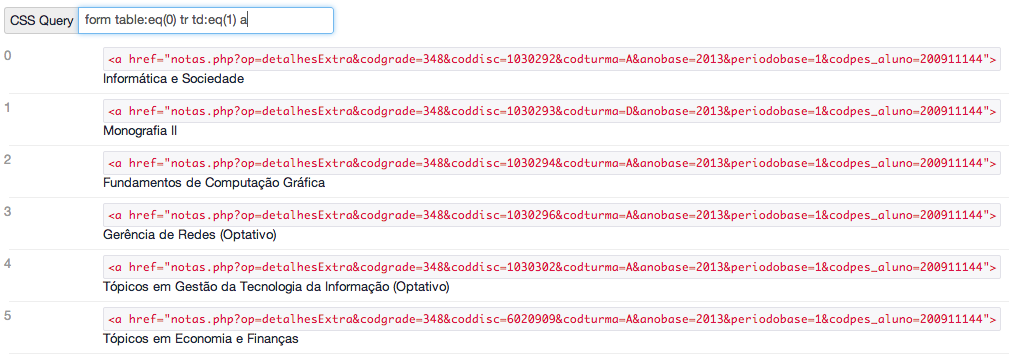
\includegraphics[scale=0.45]{imagens/listadisciplinasnotasgraduacao.png}
     \\  Fonte: Do Autor.
\end{figure}

Como pode ser percebido na Figura 9, além do nome das disciplinas, na parte em vermelho que representa a tag HTML possui o atributo \emph{href}, sendo que o mesmo armazena o link para acesso as avaliações e notas da disciplina em específico, sendo este atributo importante para a a extração das notas e avaliações das disciplinas em aberto, sendo então necessário coletar o mesmo juntamente com o nome da disciplina. Após a extração do nome das disciplinas e da respectiva url a partir do atributo \emph{href}, é iniciada a extração das avaliações por disciplina.

\subsubsection{Extração das Notas e Avaliações das Disciplinas em Aberto}
Após a extração do nome das disciplinas cursadas pelo acadêmico e da url utilizada para acesso a disciplina específica, esta mesma url é utilizada para a extração das avaliações e notas do acadêmico, assim como também das médias do graduando. Para esta extração são utilizadas várias combinações de expressões. Um exemplo de código retornado pode ser consultado na url \url{http://goo.gl/lfTy3}.

Para a extração da lista de avaliações, é utilizada a expressão \emph{form table:eq(0) tr:gt(4)} como base da extração, e posteriormente são aplicadas novas expressões sobre os resultados obtidos da aplicação da expressão base. A Figura 10 nos mostra parcialmente o retorno da expressão.

\begin{figure}[!htb]
     \centering
     \caption[Extração de Informações - Resultado parcial Avaliações]{Resultado parcial da Expressão base sobre as avaliações.}
     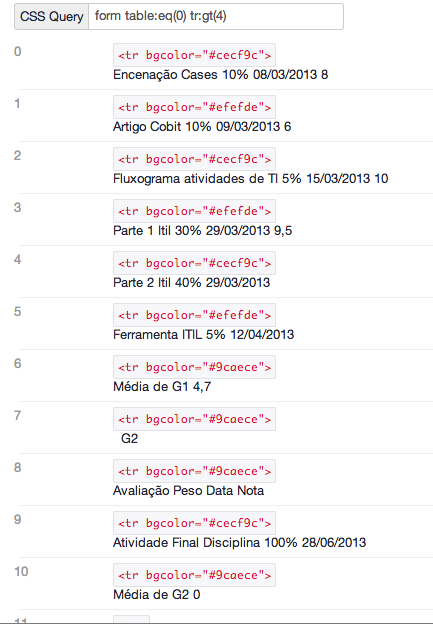
\includegraphics[scale=0.5]{imagens/avaliacoesdisciplinas1.png}
     \\  Fonte: Do Autor.
\end{figure}

Como pode ser percebido na Figura 10, as informações aparecem um pouco misturadas, sendo necessário tratar via programação as informações que realmente serão extraidas e ignorando as informações que não são necessárias. Isto é feito por meio de uma verificação de quando a informação contida na quarta coluna da tabela retornada esta em branco ou contém a palavra notas.

%\textbf{AQUI VAI O ALGORITMO DE EXTRAÇAO DAS AVALIAÇOES E NOTAS DAS DISCIPLINAS!!!!!!}

A partir do retorno acima, são extraidas as seguintes informações das avaliações: nome, peso, data e nota. Cada uma destas informações possui uma expressão aplicada sobre a expressão base. A Tabela 7 contém a expressão para cada informação e a ser extraida.

\begin{table}[!hbt]
\centering
\caption[Extração de Informações - Expressões de Extração]{Tabela de expressões de extração das informações das avaliações}
\vspace{3mm}
\begin{tabular}{p{3cm}|c}\hline
\bf{Informação} & \bf{Expressão} \\ \hline
Nome & td:eq(0)\\ \hline
Peso & td:eq(1)\\ \hline
Data & td:eq(2)\\ \hline
Nota & td:eq(3)\\ \hline
\end{tabular}
\\ Fonte: elaboração do autor.
\end{table}

Para a extração das médias de G1 e de G2 dos graduandos, são utilizadas as expressões contidas na Tabela 8, sendo que estas expressões são aplicadas diretamente sobre o código HTML, não mais sobre a expressão base.

\begin{table}[!hbt]
\centering
\caption[Extração de Informações - Extração das Médias]{Tabela de expressões de extração das médias de G1 e de G2}
\vspace{3mm}
\begin{tabular}{p{3cm}|c}\hline
\bf{Informação} & \bf{Expressão} \\ \hline
Média de G1 & form table:eq(0) tr:contains(Média de G1) td:eq(1)\\ \hline
Média de G2 & form table:eq(0) tr:contains(Média de G2) td:eq(1)\\ \hline
\end{tabular}
\\ Fonte: elaboração do autor.
\end{table}

Após estes procedimentos a extração das avaliações, assim como das médias de G1 e G2 estão concluídas, faltando apenas a extração das notas para as disciplinas já finalizadas pelo acadêmico no semestre.

\subsubsection{Extração das Notas das Disciplilas Finalizadas}
Finalizando a sessão de extração das notas da graduação, a extração das notas das disciplinas já finalizadas ocorre em cima do mesmo código HTML obtido no item 5.2.3.1 deste trabalho, que pode ser consultado na url \url{http://goo.gl/X2xJg}.

Devido a ordem em que as disciplinas são exibididas na lista de disciplinas ser diferente a ordem exibida nas notas oficiais da graduação, a expressão utilizada para a busca das notas de disciplinas já finalizadas leva em consideração o código da disciplina encerrada, extraindo o mesmo a partir do atributo href da tag html retornada na lista de disciplinas. Para o retorno das informações da disciplina já finalizada, é utilizada a expressão \emph{form[name\$=graduacao] tr:contains(CODIGODISCIPLINA)}, sendo que a palavra CODIGODISCIPLINA deve ser substituida pelo código propriamente dito.

\subsection{Horários do Semestre}
Com o objetivo de extrair o horário das disciplinas cursadas pelo acadêmico, e também as informações detalhadas da disciplina, foi desenvolvida a classe de extração dos horários do semestre. Para facilitar o entendimento, a explicação do processo será dividido em três partes, sendo elas: Extração do nome das disciplinas, Extração das informações gerais da disciplina e Extração dos Horários de Aula.

\subsubsection{Extração das Disciplinas}
Com o objetivo de extrair a lista das disciplinas pertencentes ao módulo de horários do semestre do sistema acadêmico, é necessário que a informação seja extraida a partir do código HTML retornado pela url \url{https://www.unochapeco.edu.br/saa/hor_aluno.php}. Para a obtenção das disciplinas corretas cursadas pelo acadêmico, é utilizado o cookie de sessão capturado no momento do login, conforme explicado no item 5.2.1 deste trabalho. Um exemplo de código HTML retornado pelo servidor a partir deste tipo de consulta pode ser visto na url \url{http://goo.gl/kz9NN}.

A partir do código HTML retornado, utilizando-se das expressões exibidas na Tabela 9 são extraidas as informações de código, nome e turma da disciplina.

\begin{table}[!hbt]
\centering
\caption[Extração de Informações - Expressões de Extração Horários do Semestre]{Tabela de expressões de extração dos horários do semestre.}
\vspace{3mm}
\begin{tabular}{p{3cm}|c}\hline
\bf{Informação} & \bf{Expressão}           \\ \hline
Código          & form tr:gt(1) td:eq(0) a \\ \hline
Nome            & form tr:gt(1) td:eq(1) a \\ \hline
Turma           & form tr:gt(1) td:eq(2) a \\ \hline
\end{tabular}
\\ Fonte: elaboração do autor.
\end{table}

%\textbf{VERIFICAR COM O MC SE DEVEM SER COLOCADAS IMAGENS AQUI!!!}

Como ocorre na extrações anteriores, é necessário extrair da tag HTML retornada o atributo \emph{href} para serem extraidas tanto as informações gerais como os horários de aula da disciplina.

Após terminada a extração das disciplinas, e possuindo a url armazenada no atributo \emph{href}, agora são extraidas as informações gerais das disciplinas e também os horários de aula.

\subsubsection{Extração das Informações Gerais}
A extração das Informações gerais ocorre a partir da url extraida da disciplina como visto no item 5.2.4.1 deste trabalho. Para a extração das informarmações é necessária uma expressão para cada informação, sendo demonstradas as expressões na tabela 10. O código HTML retornado pela página do sistema acadêmico para uma disciplina de exemplo pode ser consultado na url \url{http://goo.gl/auHL8}.

\begin{table}[!hbt]
\centering
\caption[Extração de Informações - Expressões de Extração dos Detalhes da Disciplina]{Tabela de expressões de extração dos detalhes das disciplinas.}
\vspace{3mm}
\begin{tabular}{p{3cm}|c}\hline
\bf{Informação} & \bf{Expressão}                                 \\ \hline
Curso           & form tr[bgcolor]:contains(curso) td:eq(1)      \\ \hline
Grade           & form tr[bgcolor]:contains(grade) td:eq(1)      \\ \hline
Disciplina      & form tr[bgcolor]:contains(disciplina) td:eq(1) \\ \hline
Período         & form tr[bgcolor]:contains(período) td:eq(1)    \\ \hline
Professor       & form tr[bgcolor]:contains(professor) td:eq(1)  \\ \hline
Turno           & form tr[bgcolor]:contains(turno) td:eq(1)      \\ \hline
Créditos        & form tr[bgcolor]:contains(créditos) td:eq(1)   \\ \hline
Data da G2      & form tr[bgcolor]:contains(g2) td:eq(1)         \\ \hline
Data da G3      & form tr[bgcolor]:contains(g3) td:eq(1)         \\ \hline
\end{tabular}
\\ Fonte: elaboração do autor.
\end{table}

%\textbf{VERIFICAR COM O MC SE DEVEM SER COLOCADAS IMAGENS COM OS DETALHES EXTRAIDOS AQUI!!!!}

A partir de cada uma das expressões presentes na Tabela 10, obtemos cada uma das informações que fazem parte dos detalhes da disciplina cursada pelo acadêmico, e desta forma encerramos a extração dos detalhes, iniciando a extração dos horários de aula explicada no item 5.2.4.3.

\subsubsection{Extração dos Horários de Aula}
Como última parte da extração das informações, falaremos da Extração dos horários de aula. Tendo como base a mesma url e código HTML utilizado no item 5.2.4.2 deste trabalho, podemos obter os horários de aula das disciplinas. Para isso é aplicada a expressão \emph{form table:eq(1) tr:gt(1)} que nos retorna a lista com as aulas da disciplina, conforme pode ser visto na Figura 11.

\begin{figure}[!htb]
     \centering
     \caption[Extração de Informações - Horários do Semestre]{Lista de horários para uma disciplina.}
     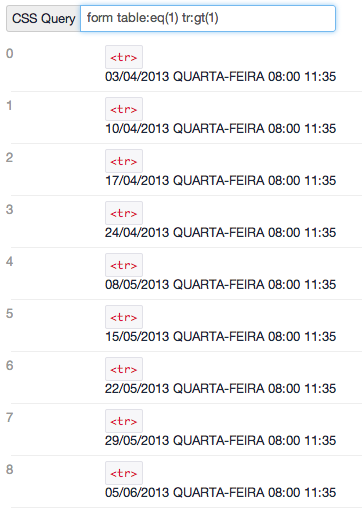
\includegraphics[scale=0.5]{imagens/listahorariossemestre.png}
     \\  Fonte: Do Autor.
\end{figure}

%\newpage

A partir do retorno da expressão demonstrado na Figura 11, são aplicadas novas expressões para obter-se as informações específicas necessárias, sendo estas expressões mostradas na Tabela 11.

\begin{table}[!hbt]
\centering
\caption[Extração de Informações - Expressões de Extração dos Detalhes da Disciplina]{Tabela de expressões de extração dos detalhes das disciplinas.}
\vspace{3mm}
\begin{tabular}{p{3cm}|c}\hline
\bf{Informação} & \bf{Expressão}                                 \\ \hline
Data            & td:eq(0) \\ \hline
Dia da Semana   & td:eq(1) \\ \hline
Hora            & td:eq(2) \\ \hline
Ocorreu         & b        \\ \hline
\end{tabular}
\\ Fonte: elaboração do autor.
\end{table}

Para saber se a aula já foi ministrada ou não, é validado se a informação sendo extraida está em negrito no código HTML, acrescentando-se a expressão \emph{b} a expressão original.

Desta forma, toda a extração de informações utilizando a biblioteca \emph{jsoup} é finalizada, sendo necessário agora preprar o arquivo que será enviado ao aplicativo móvel utilizando o servidor REST.

\section{Preparação dos Dados}
A preparação dos dados para o envio para a aplicação móvel é feita em conjunto com a extração dos dados da página, porém para demonstrar de forma mais simples e facilitar o entendimento este capítulo irá demonstrar apenas o layout dos arquivos gerados. 

Toda a geração dos arquivos funciona como retorno das funções de extração, sendo que o retorno ocorre em formato JSON, devido ao formato simples de representação de dados e economia da banda de dados se comparado com o formato XML, já que o JSON não possui tags de fechamento e cabeçalho nos arquivos. Não existe muitas coisas a serem explicadas sobre os arquivos gerados, pois os mesmos são de fácil leitura e entendimento, e juntamente com as informações já comentadas no item 5.2 deste trabalho causaria redundância nas informações.

\section{Servidor REST}
Após extração e preparação dos dados, resta apenas disponibilizar as informações para acesso externo. Para esta tarefa foi utilizada a classe Icebreak REST Server \cite{IcebreakRestServer}, que implementa um servidor REST básico que atende as necessidades deste trabalho. Foi necessária apenas uma alteração no cabeçalho HTML retornado pela classe, o qual retornava tamanhos errados, que acabavam ocasionando a perda de informações do arquivo JSON. Como não é um parâmetro obrigatório do cabeçalho do HTML, o tamanho deixou de ser enviado no mesmo, e assim o problema deixou de existir (o código-fonte da implementação da classe com a alteração do cabeçalho pode ser conferida no Apêndice C). 

Como todo serviço de rede, é necessário escutar uma porta para receber as conexões, e neste trabalho foi escolhida a porta 90 para o servidor REST, pois assim não ocasionaria um conflito com a porta 80 utilizada pelos servidores HTTP.

Como possuimos três tipos de retorno no servidor, cada um referente a um módulo do sistema acadêmico, para otimizar o envio e também otimizar a extração no lado da aplicação, foram utilizados parâmetros na URL utilizada para conectar ao servidor, sendo estes parâmetros demonstradas na tabela 12.

\begin{table}[!hbt]
\centering
\caption[Servidor REST - Parâmetros do Servidor]{Tabela com os parâmetros aceitos pelo servidor REST.}
\vspace{3mm}
\begin{tabular}{p{3cm}|p{9cm}}\hline
\textbf{Parâmetro} & \textbf{Descrição} \\ \hline
usuario            & Neste parâmetro é possível passar ao servidor tanto a matrícula do acadêmico como o seu email da Unochapecó. Parâmetro Obrigatório  \\ \hline
senha              & Neste parâmetro deve ser informada a senha do acadêmico referente a matrícula ou email informado. Parâmetro Obrigatório. \\ \hline
info               & Neste campo é passado o tipo de informação que deseja ser recebida do servidor. \\ \hline
\end{tabular}
\\ Fonte: elaboração do autor.
\end{table}

O parâmetro \emph{info} presente na Tabela 12 merece uma atenção especial, pois o mesmo não é obrigatório. Caso o mesmo seja omitido da URL de conexão com o servidor, teremos como retorno um valor booleano informando se o login é válido. Nesta implementação do servidor, são três as possíveis opções para o parâmetro \emph{info}: materiais, notas e horarios. Cada uma das opções refere-se a um dos módulos do sistema acadêmico extraidos anteriormente.

O acesso ao servidor ocorre por meio de requisições HTTP na porta 90. Por exemplo, caso se deseje se obter as informações do material de apoio de determinado acadêmico com o nome de usuário \emph{teste} e a senha \emph{teste}, e o servidor estivesse rodando localmente na máquina utilizada para consulta, bastaria utilizar a URL \url{http://localhost:90?usuario=teste&senha=teste&info=materiais}, sendo assim o servidor encarregado de validar o login e retornar as informações corretas referentes aos materiais de apoio do acadêmico.
\chapter{Aplicação}

% Referencias - SQLite, JSON, APPCELERATOR TITANIUM, JavaScript, SQL

Tendo como base o questionário apresentado anteriormente onde obtemos maior quantidade de respostas referentes aos acadêmicos de cursos de graduação, foi decidido para este trabalho implementar a aplicação para este público alvo, sendo implementados os módulos que apresentaram as três melhores notas, sendo eles Material de Apoio, Notas da Graduação e Horários do Semestre.

Para o desenvolvimento da aplicação, foi utilizado exclusivamente a ferramenta de desenvolvimento \emph{Titanium SDK} desenvolvida pela \emph{Appcelerator Inc.} devido ao fato de a mesma ser gratuita e utilizar uma linguagem com curva de aprendizado suave. Além disso o fato de utilizar a mesma e desenvolver em JavaScript utilizando ela facilitou a comunicação com o servidor e a extração dos arquivos JSON retornados por ele. Além disso, utilizando-se o \emph{Titanium SDK} para o desenvolvimento, é possível compilar com o mesmo código fonte aplicações para Android e iOS, plataformas mais utilizadas pelos acadêmicos da instituição. Apesar de ser fortemente lembrados os padrões, nem todo o sistema foi desenvolvido utilizando-se os conceitos de orientação a objetos, sendo utilizadas tanto técnicas de programação estruturada como orientação a objetos conforme a técnica que melhor atendia o desenvolvimento do módulo em específico.

Todas as informações extraidas do servidor são inseridas em uma base de dados SQLite no próprio dispositivo, possibilitando assim a consulta offline das informações.

Para facilitar e modularizar este capítulo, as informações referentes a cada módulo foram separadas em sessões que serão apresentadas a seguir.

\section{Base de Dados da Aplicação}

Com o objetivo de armazenar as informações enviadas pelo servidor, foi modelada uma pequena base de dados composta por 5 tabelas utilizadas no armazenamento de dados e uma tabela para armazenamento das configurações. Para esta base de dados foi utilizado o SQLite, nativo nos dispositivos Android e iOS.

\subsection{Tabela de Configuração}
A tabela de configuração é a única tabela não transmitida pelo servidor para a aplicação, sendo gerada e manipulada no próprio dispositivo. A lista de campos e seus respectivos tipos de dados é demonstrada na Tabela 13.

\begin{table}[!hbt]
\centering
\caption[Aplicação - Tabela de Configuração]{Layout da tabela de configuração}
\vspace{3mm}
\begin{tabular}{c|c}\hline
\textbf{Nome do Campo} & \textbf{Tipo de Dados} \\ \hline
login & TEXT \\ \hline
senha & TEXT \\ \hline
\end{tabular}
\\ Fonte: elaboração do autor.
\end{table}

Como pode ser visto, é uma tabela simples que armazena as informações de login, sendo estas utilizadas no para o recebimento das informações atualizadas de dentro do sistema.

\subsection{Tabela de Material de Apoio}
A tabela de Material de apoio é extraida a partir do arquivo JSON de materiais transmitido pelo servidor, e é responsável por armazenar a lista de materiais para todas as disciplinas cursadas pelo acadêmico que está utilizando o aplicativo. Os campos e tipos de dados podem ser consultados na Tabela 14.

\begin{table}[!hbt]
\centering
\caption[Aplicação - Tabela de Material de Apoio]{Layout da tabela de Material de Apoio}
\vspace{3mm}
\begin{tabular}{c|c}\hline
\textbf{Nome do Campo} & \textbf{Tipo de Dados} \\ \hline
nomeDisciplina         & TEXT                   \\ \hline
publicacao             & TEXT                   \\ \hline 
nome                   & TEXT                   \\ \hline
descricao              & TEXT                   \\ \hline
url                    & TEXT                   \\ \hline
\end{tabular}
\\ Fonte: elaboração do autor.
\end{table}

Devido a quantidade de colunas ser reduzida, as informações dos materiais de apoio foi a única que não foi dividida em duas tabelas, sendo possível manter sem problemas as informações em apenas uma tabela, não gerando grande duplicidade nas informações.

\subsection{Tabela de Horários do Semestre}
Com o objetivo de facilitar as consultas SQL executadas na base de dados e fornecer uma complexidade menor na leitura do código, o JSON de Horários do Semestre retornado pelo servidor é extraido em duas tabelas unidas por uma chave. Desta forma, a tabela de Horários do Semestre é responsável pelo armazenamento das disciplinas e seus detalhes. Na Tabela 15 pode-se observar a lista dos campos e seus respectivos tipos.

\begin{table}[!hbt]
\centering
\caption[Aplicação - Tabela de Horários do Semestre]{Layout da tabela de Horários do Semestre}
\vspace{3mm}
\begin{tabular}{c|c}\hline
\textbf{Nome do Campo} & \textbf{Tipo de Dados} \\ \hline
codigo                 & TEXT                   \\ \hline
turma                  & TEXT                   \\ \hline
nome                   & TEXT                   \\ \hline
curso                  & TEXT                   \\ \hline
dataG2                 & TEXT                   \\ \hline
dataG3                 & TEXT                   \\ \hline
professor              & TEXT                   \\ \hline
creditos               & INTEGER                \\ \hline
turno                  & TEXT                   \\ \hline
grade                  & INTEGER                \\ \hline
periodo                & INTEGER                \\ \hline
\end{tabular}
\\ Fonte: elaboração do autor.
\end{table}

\subsection{Tabela de Horários do Semestre por Disciplina}
Responsável por armazenar as informações dos horários das aulas e se as mesmas já ocorreram, esta tabela pode ser considerada uma extenção da tabela de Horários do Semestre, sendo ligada a mesma pelos campos código e turma. Na Tabela 16 são representados todos os campos da tabela e seus respectivos dados.

\begin{table}[!hbt]
\centering
\caption[Aplicação - Tabela de Horários do Semestre por Disciplina]{Layout da tabela de Horários do Semestre por Disciplina}
\vspace{3mm}
\begin{tabular}{c|c}\hline
\textbf{Nome do Campo} & \textbf{Tipo de Dados} \\ \hline
codigo                 & TEXT                   \\ \hline
turma                  & TEXT                   \\ \hline
hora                   & TEXT                   \\ \hline
diasemana              & TEXT                   \\ \hline
data                   & TEXT                   \\ \hline
ocorreu                & TEXT                   \\ \hline
\end{tabular}
\\ Fonte: elaboração do autor.
\end{table}

\subsection{Tabela de Notas da Graduação}
Com o objetivo de facilitar as consultas SQL executadas na base de dados e fornecer uma complexidade menor na leitura do código, o JSON de Notas da Graduação retornado pelo servidor é extraido em duas tabelas unidas por uma chave. Desta forma, a tabela de Notas da Graduação é responsável pelo armazenamento das disciplinas e seus detalhes. Na Tabela 17 pode-se observar a lista dos campos e seus respectivos tipos.

\begin{table}[!hbt]
\centering
\caption[Aplicação - Tabela de Notas da Graduação]{Layout da tabela de Notas da Graduação}
\vspace{3mm}
\begin{tabular}{c|c}\hline
\textbf{Nome do Campo} & \textbf{Tipo de Dados} \\ \hline
nome                   & TEXT                   \\ \hline
notaG1                 & FLOAT                  \\ \hline
notaG3                 & FLOAT                  \\ \hline
notaG2                 & FLOAT                  \\ \hline
mediaFinal             & FLOAT                  \\ \hline
estadoMateria          & TEXT                   \\ \hline
statusAcademico        & TEXT                   \\ \hline
\end{tabular}
\\ Fonte: elaboração do autor.
\end{table}

\subsection{Tabela de Avaliações}
Responsável por armazenar as informações das avaliações já minstradas, esta tabela pode ser considerada uma extenção da tabela de Notas da Graduação, sendo ligada a mesma pelo campo nome. Na Tabela 18 são representados todos os campos da tabela e seus respectivos dados.
    
\begin{table}[!hbt]
\centering
\caption[Aplicação - Tabela de Avaliações]{Layout da tabela de Avaliações}
\vspace{3mm}
\begin{tabular}{c|c}\hline
\textbf{Nome do Campo} & \textbf{Tipo de Dados} \\ \hline
nomeDisciplina         & TEXT                   \\ \hline
peso                   & TEXT                   \\ \hline
nota                   & FLOAT                  \\ \hline
data                   & TEXT                   \\ \hline 
nome                   & TEXT                   \\ \hline
\end{tabular}
\\ Fonte: elaboração do autor.
\end{table}

\section{Conexão ao Servidor e Extração dos Dados}
A conexão com o servidor ocorre conforme explicado no item 5.4 deste trabalho, onde a partir de uma URL utilizando-se de um cliente HTTP para a conexão. Para o sincronismo das aplicações móveis, foi criado um servidor utilizando-se do endereço \url{http://minhaunomovel.no-ip.org}, sendo então necessário utilizar este endereço na montagem da URL de extração das informações. Os passos para conexão e extração dos dados estão representados no \emph{Apêndice B.1}.

O processo de conexão com o servidor e de extração de dados ocorrem em conjunto onde a partir da conexão, caso a informação buscada seja retornada é chamada a função de extração de dados, que efetua a conversão do JSON transmitido pelo servidor em um objeto JavaScript, e posteriormente extrai as informações e insere as mesmas na base de dados. 

Após o recebimento do arquivo JSON referente ao módulo do sistema a ser extraido, o arquivo JSON é convertido para um objeto nativo JavaScript, sendo que sua manipulação se da de forma extremamente simples, onde os vetores anteriormente representados no JSON agora são acessados como vetores da linguagem, e os objetos se tornam objetos realmente, sem necessidade de funções especiais para acessar seus dados. Desta forma, conforme pode ser visto no \emph{Apêndice B.1} as informações preenchidas no objeto JSON são acessadas sem utilização de funções especiais de acesso e inseridas diretamente na base de dados SQLite.

\section{Login e Persistência das Informações}
Sendo o formulário de entrada do sistema, o formulário de login é a ``porta de entrada'' do acadêmico, sendo por meio deste feito a validação dos dados de login, e posteriormente o recebimento das informações. Na Figura 13 pode ser vista a interface deste formulário.

\begin{figure}[!htb]
     \centering
     \caption[Formulário de Login - Interface]{Interface do Formulário de Login}
     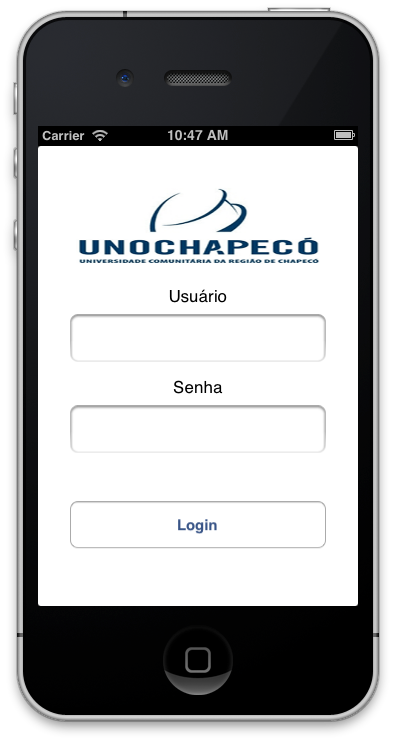
\includegraphics[scale=0.34]{imagens/formlogin.png}
     \\  Fonte: Do Autor.
\end{figure}

Com o objetivo de ser um formulário simples, foi pensado em uma interface limpa, apenas com as informações necessárias. Desta forma o layout a cima foi o escolhido, apenas com os campos de usuário e senha, a logo da instituição e um botão de login.

Após inseridas as informações, no momento que é acionado o botão de login, a aplicação conecta-se com o servidor e recebe os dados do acadêmico. Também neste momento as informações de login e senha são armazenadas na tabela de configuração, sendo que exceto quando o usuário efetua logout (opção sair do menu principal da apliçação), o formulário de login não é mais exibido ao usuário, sendo feito o login de forma automática.

A implementação deste formulário pode ser consultada no \emph{Apêndice B.2}.

\section{Formulário Principal}

Sendo o menu principal da aplicação o formulário principal é a tela de escolha do usuário, onde o mesmo pode acessar os outros menus da aplicação. Seguindo a idéia de simplicidade proposta, utiliza-se de uma lista de opções possuindo acima desta lista a logo da instituição, como pode ser visto na Figura 14.

\begin{figure}[!htb]
     \centering
     \caption[Formulário Principal - Interface]{Interface do Formulário Principal do Aplicativo.}
     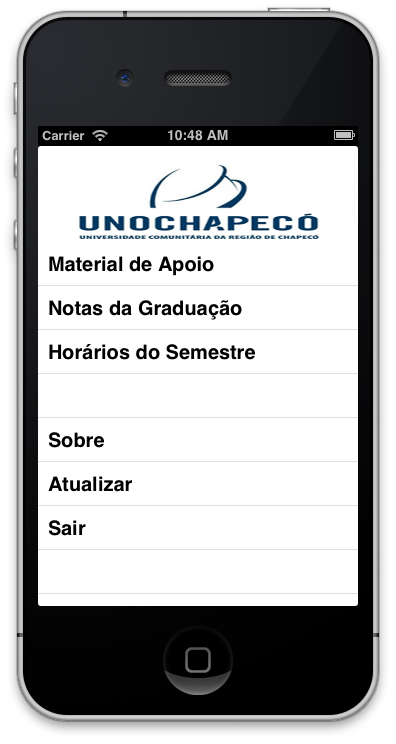
\includegraphics[scale=0.34]{imagens/formprincipal.png}
     \\  Fonte: Do Autor.
\end{figure}

A partir do formulário principal, o usuário pode ser levado para qualquer formulário da aplicação. A opção ``Sobre'' exibe um alerta mostrando mais informações sobre a apliçação, conforme pode ser visto na Figura 15.

\begin{figure}[!htb]
     \centering
     \caption[Formulário Principal - Sobre]{Informações sobre o Aplicativo.}
     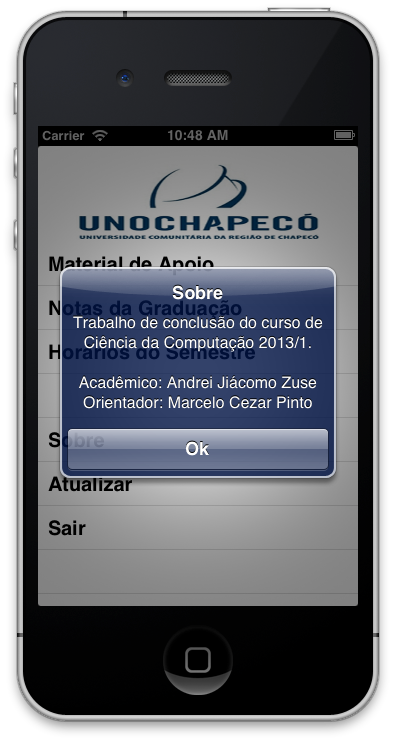
\includegraphics[scale=0.34]{imagens/formsobre.png}
     \\  Fonte: Do Autor.
\end{figure}
\newpage

A opção ``Atualizar'' exibida no menu principal é utilizada pelo usuário para receber novos dados do servidor, sendo assim atualizadas as informações armazenadas no dispositivo. Já a opção ``Sair'' é utilizada para fazer logout do sistema, excluindo as informações armazenadas na base de dados do aplicativo e retornando ao formulário de login.

A implementação deste formulário pode ser consultada no \emph{Apêndice B.3}.


\section{Material de Apoio}
Desenvolvido com o objetivo de permitir a consulta da lista de materiais de apoio das disciplinas, e também permitir visualizar o material (desde que haja suporte pelo dispositivo para visualização do material disponibilizado). Na Figura 16 é possível visualizar o layout da interface gráfica do módulo.

\begin{figure}[!htb]
     \centering
     \caption[Formulário Material de Apoio - Interface]{Interface do Formulário de Material de Apoio.}
     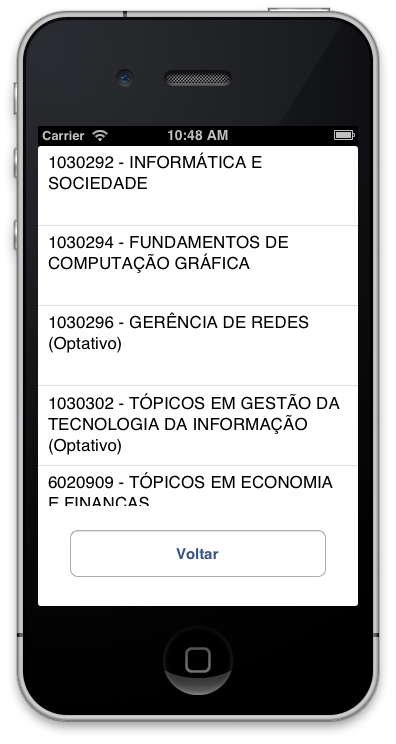
\includegraphics[scale=0.34]{imagens/formmaterialapoio.png}
     \\  Fonte: Do Autor.
\end{figure}

Ao ser selecionada alguma disciplina, a lista dos materiais da mesma é exibida. Para a Figura 17 foi selecionada a disciplina de Informática e Sociedade, carregando assim a lista de materiais da mesma.

\begin{figure}[!htb]
     \centering
     \caption[Formulário Material de Apoio - Consulta de Materiais]{Interface do Formulário de Consulta de Materiais.}
     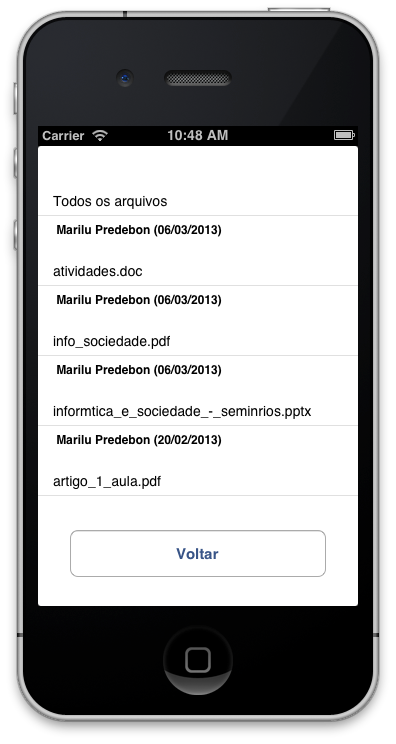
\includegraphics[scale=0.34]{imagens/formmaterialdisciplina.png}
     \\  Fonte: Do Autor.
\end{figure}
\newpage

Ao se escolher uma disciplina, o navegador do dispositivo é chamado, para abrir o material escolhido pelo usuário. Neste ponto é solicitado o login do acadêmico no sistema acadêmico pelo browser, pois não possuímos acesso a sessão em que o arquivo foi extraido no servidor. Após o login, material é exibido, conforme Figura 18.

\begin{figure}[!htb]
     \centering
     \caption[Formulário Material de Apoio - Visualização de Material]{Visualização do Material de Apoio selecionado pelo usuário.}
     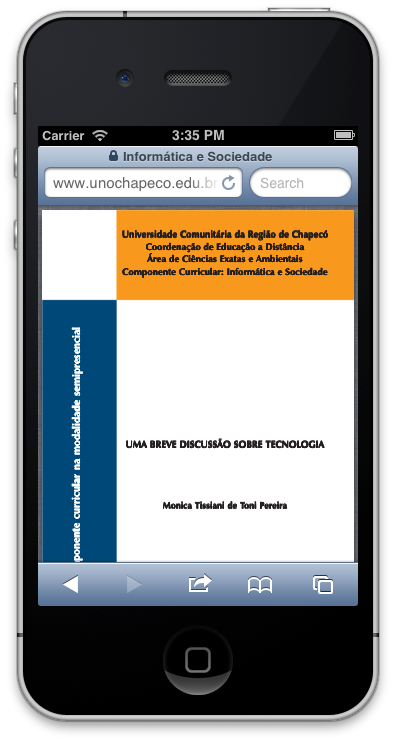
\includegraphics[scale=0.34]{imagens/visualizacaomaterialapoio.png}
     \\  Fonte: Do Autor.
\end{figure}
\newpage

A implementação dos formulários de exibição das disciplinas e dos materiais podem ser consultados nos Apêndices \emph{B.4} e \emph{B.5}.

\section{Notas da Graduação}
O formulário de Notas da Graduação é a interface do usuário para visualização, a partir das disciplinas cursadas pelo mesmo, visualizar suas médias e suas notas por avaliação. Sua interface incial, assim como os outros formulários de consulta, consiste na lista das disciplinas cursadas pelo acadêmico, conforme Figura 19.

\begin{figure}[!htb]
     \centering
     \caption[Formulário Notas da Graduação - Lista das Disciplinas]{Visualização do Formulário de Notas da Graduação.}
     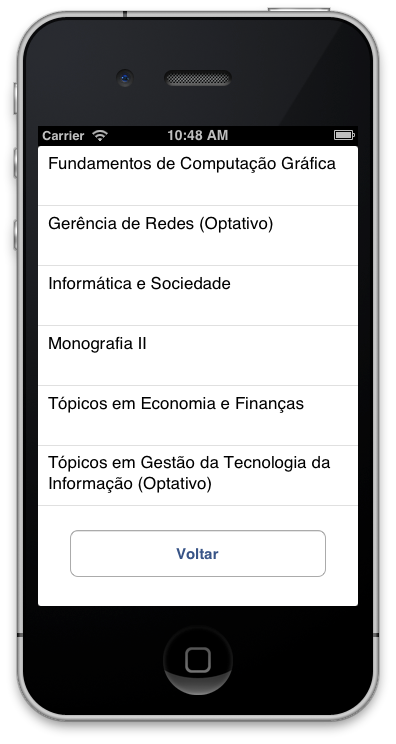
\includegraphics[scale=0.34]{imagens/formnotasgraduacao.png}
     \\  Fonte: Do Autor.
\end{figure}
\newpage

Ao selecionar uma disciplina, é apresentada uma tela com as médias do acadêmico. Caso a disciplina esteja aberta, a tela exibida é semelhante a visualizada na Figura 20. Já caso a disciplina ainda esteja aberta, a imagem exibida é semelhante a Figura 21, exibindo o botão detalhes para a consulta das avaliações feitas pelo acadêmico.

\begin{figure}[!htb]
     \centering
     \caption[Formulário Notas da Graduação - Visualização de Disciplina Fechada]{Visualização das notas de uma disciplina fechada.}
     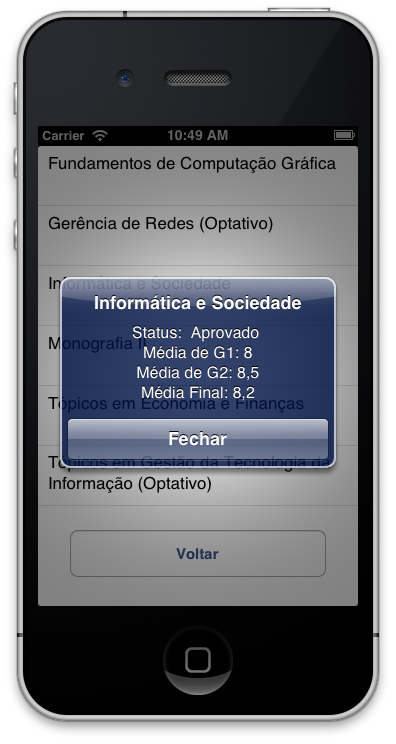
\includegraphics[scale=0.34]{imagens/formvisualizacaomediassemdetalhes.png}
     \\  Fonte: Do Autor.
\end{figure}
\begin{figure}[!htb]
     \centering
     \caption[Formulário Notas da Graduação - Visualização de Disciplina Aberta]{Visualização das notas de uma disciplina em aberto.}
     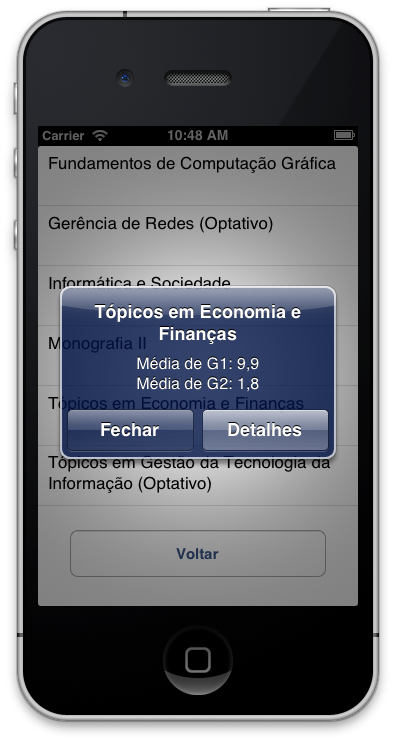
\includegraphics[scale=0.34]{imagens/formvisualizacaomediascomdetalhes.png}
     \\  Fonte: Do Autor.
\end{figure}
\newpage

Em caso de disciplina em aberto, onde o botão ``Detalhes'' é exibido, ao ser escolhio pelo usuário é exibida a tela de avaliações, que mostra as informações referentes as avaliações, caso as mesmas existam (Figura 22), ou é exibida uma mensagem informando que não existem avaliações (Figura 23).

\begin{figure}[!htb]
     \centering
     \caption[Formulário Notas da Graduação - Visualização de Atividades]{Visualização das atividades e suas informações.}
     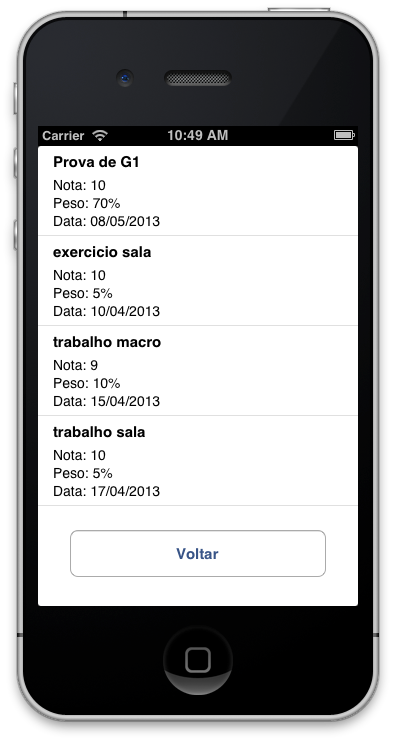
\includegraphics[scale=0.34]{imagens/formatividades.png}
     \\  Fonte: Do Autor.
\end{figure}
\begin{figure}[!htb]
     \centering
     \caption[Formulário Notas da Graduação - Inexistência de Avaliações]{Alerta sobre não existirem avaliações cadastradas no sistema acadêmico.}
     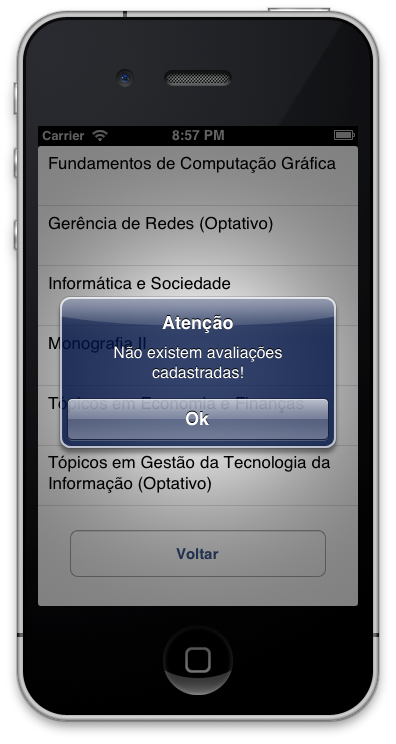
\includegraphics[scale=0.34]{imagens/alertanaoexistemavaliacoes.png}
     \\  Fonte: Do Autor.
\end{figure}

A implementação dos formulários de exibição das disciplinas e das avaliações podem ser consultados nos Apêndices \emph{B.6} e \emph{B.7}.

\section{Horários do Semestre}
O formulário de horários do semestre exibe tanto informações detalhadas sobre a disciplina cursada pelo acadêmico como também os dias de aula da disciplina. Ao ser acessado, assim como os outros formulários, é exibida a lista das disciplinas cursadas, conforme mostrado na Figura 24.
\begin{figure}[!htb]
     \centering
     \caption[Formulário Horários do Semestre - Lista das Disciplinas]{Visualização do Formulário de Horários do Semestre.}
     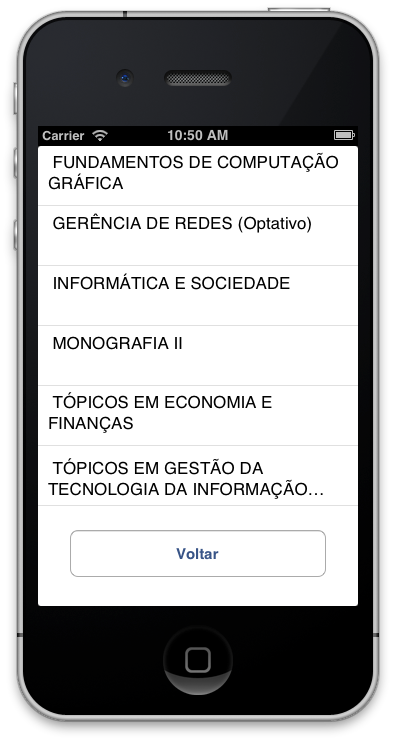
\includegraphics[scale=0.34]{imagens/formhorariosemestre.png}
     \\  Fonte: Do Autor.
\end{figure}

Ao selecionar uma disciplina na lista apresentada, é exibido ao acadêmico um alerta com as informações da disciplina (Figura 25) e também um botão detalhes, que exibe a lista completa de datas e horários de aula da disciplina escolhida (Figura 26).

\begin{figure}[!htb]
     \centering
     \caption[Formulário Horários do Semestre - Visualização de Informações]{Visualização dos detalhes da disciplina selecionada.}
     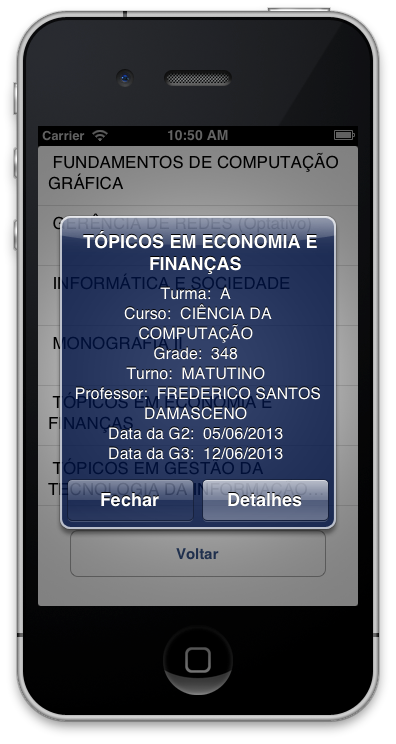
\includegraphics[scale=0.34]{imagens/formhorariossemestredetalhes.png}
     \\  Fonte: Do Autor.
\end{figure}
\begin{figure}[!htb]
     \centering
     \caption[Formulário Horários do Semestre - Visualização dos Horários]{Visualização das datas e horários de aula.}
     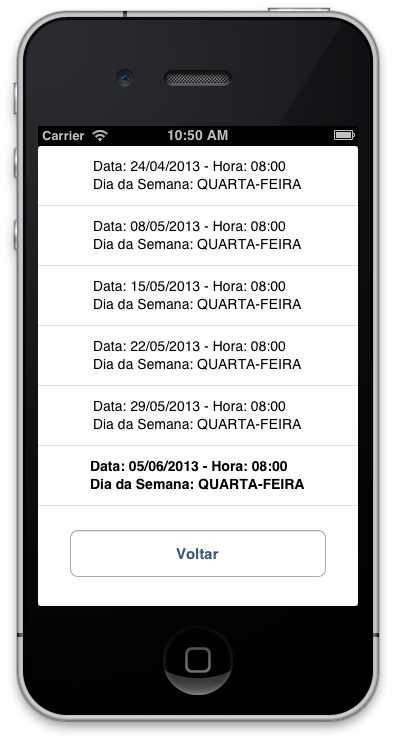
\includegraphics[scale=0.34]{imagens/formconsultahorariosemestredisciplina.png}
     \\  Fonte: Do Autor.
\end{figure}
\newpage

Conforme pode ser visto na Figura 26, o último registro é exibido em destaque. Isto significa que a aquela aula ainda não foi realizada, assim como ocorre no sistema acadêmico Minha Uno.

A implementação dos formulários de exibição das disciplinas e dos horários podem ser consultados nos Apêndices \emph{B.8} e \emph{B.9}.

\section{Execução no Google Android}

\chapter{Conclusão}

Este trabalho mostrou que é de interesse da comunidade acadêmica da instituição um aplicativo para dispositivos móveis, e que o desenvolvimento do mesmo também é possível. Este trabalho também mostra que mesmo não possuindo acesso direto as bases de dados computacionais de uma instituição, a partir de visões ou conexões a tabelas, é possível obter-se as informações do sistema acadêmico utilizando os meios onde as informações convencionalmente são disponibilizadas, neste caso, uma página da internet. Mesmo não sendo a melhor prática, com esforço e aplicação de conceitos é possível a obtenção dos dados desejados.

Apesar da falta de apoio da diretoria de T.I. da instituição para fornecimento das informações e infra-estrutura, com a utilização de métodos de extração e o esforço para entender o funcionamento da página web do sistema acadêmico foi possível extrair as informações utilizando algumas vulnerabilidades do sistema acadêmico atual para isso. Sem estas vulnerabilidades exploradas (como por exemplo o sistema de login utilizado) o trabalho tornaria-se mais difícil, e quem sabe não fosse possível obter as informações do sistema acadêmico Minha Uno.

Além disso, apesar das diversas tentativas de envio do questionário a toda a instituição, para assim obter-se dados conclusivos sobre todos os módulos do sistema acadêmico, apenas os estudantes de graduação da Área de Ciências Exatas e Ambientais receberam o questionário, desta forma não sendo possível atingir toda a instituição, principalmente o corpo de docentes, que posteriormente ao questionário ficaram sabendo da existência do mesmo.

Porém apesar de todas as dificuldades, o trabalho mostrou tanto a possibilidade de extrair-se as informações e implementar uma aplicação móvel, como também serviu de fonte de conhecimento para trabalhos similares, onde é possível, consultando-se este trabalho, serem desenvolvidos outros meios de integração ou novas aplicações para o sistema acadêmico Minha Uno, partindo-se da experiência obtida com esta aplicação para dispositivos móveis.

\section{Trabalhos Futuros}

Devido ao grau de complexidade do projeto não foi possível implementar todos os módulos do sistema acadêmico Minha Uno. Desta forma seria interessante a continuidade do projeto, implementando os módulos faltantes do perfil de graduação, e os outros perfis faltantes.

Para seguir as tendências de design atuais, seria muito interessante a adoção do design "flat" na aplicação, implementando desta forma uma interface gráfica mais atrativa aos usuários.

Como este trabalho depende do layout do arquivo HTML do sistema acadêmico atual, caso o sistema acadêmico sofra alterações de layout é necessária manutenção no servidor, adequando a extração dos dados ao novo layout do arquivo HTML.

Com o objetivo de a aplicação tornar-se opensource e poder atingir outras universidades, seria interessante padronizar a integração da aplicação e melhorar a sua abstração, possibilitando assim as universidades a partir do projeto base, sem muitas alterações no mesmo, poderem utilizar a aplicação para benefício dos seus acadêmicos.

Implementar notificações automáticas na aplicação, para avisar os usuários quando ocorre alguma alteração nos dados do mesmo, como o recebimento de um novo material ou uma nova nota cadastrada no sistema acadêmico.

Como dados são transmitidos entre o servidor e a aplicação, é necessário implementar medidas de segurança, para que os dados não possam ser interceptados no momento do sincronismo.

\bibliography{bibliografia}
\appendix
\chapter{Servidor}
\lstset{
    language=java,
    basicstyle=\scriptsize,
    upquote=true,
    aboveskip={1.5\baselineskip},
    columns=fullflexible,
    showstringspaces=false,
    extendedchars=true,
    breaklines=true,
    showtabs=false,
    showspaces=false,
    showstringspaces=false,
    frame=single,
    literate={á}{{\'a}}1 {ã}{{\~a}}1 {é}{{\'e}}1 {ç}{{\c{c}}}1 {Ç}{{\c{C}}}1 {Ã}{{\~A}}1 {Í}{{\'I}}1 {Ó}{{\'O}}1 {â}{{\^a}}1 {í}{{\'i}}1
}

Abaixo serão apresentados os códigos desenvolvidos para o servidor que oferece suporte a aplicação.

\section{Login.java}
\begin{lstlisting}[language=java, frame=single]
package edu.unochapeco.saa;

import java.io.IOException;
import org.jsoup.Connection;
import org.jsoup.Jsoup;
import org.jsoup.nodes.Document;

public class Login {

    private String session = null;
    
    
    public boolean connect(String user, String pass) throws IOException 
    {
        String url = "https://www.unochapeco.edu.br/usuarios/login";

        if (this.session == null) {
            Connection.Response response = Jsoup.connect(url)
                    .data("login_submited", "1",
                    "usuario", user,
                    "senha", pass,
                    "submit", "entrar")
                    .method(Connection.Method.POST)
                    .execute();
            
            this.session = response.cookie("PHPSESSID");
        }
        
         //Testa se o login foi bem sucedido
            Document document = Jsoup.connect(url)
                .cookie("PHPSESSID", this.session)
                .get();

        return !document.text().contains("GRADUAÇÃO PÓS BOLSAS NOTÍCIAS UNOWEBTV "
                + "EVENTOS INSTITUCIONAL MINHA UNO WEBMAIL CONTATO");
        
        
    }

    public String getSession() throws IOException {
        
        return this.session;
    }
}
\end{lstlisting}

\section{MaterialApoio.java}
\begin{lstlisting}[language=java, frame=single]
package edu.unochapeco.saa;

import java.io.IOException;
import org.json.JSONArray;
import org.json.JSONObject;
import org.jsoup.Jsoup;
import org.jsoup.nodes.Document;
import org.jsoup.nodes.Element;
import org.jsoup.select.Elements;

public class MaterialApoio {

    private String session = null;

    public MaterialApoio(String session) {
        this.session = session;
    }

    public String getMateriais() throws IOException {
        String url = "https://www.unochapeco.edu.br/saa/materialApoio.php";

        Document document = Jsoup.connect(url)
                .cookie("PHPSESSID", session)
                .timeout(8000)
                .get();

        Elements disciplinas = document.select("form tr td:eq(1) a");

        JSONArray disciplinaArray = new JSONArray();
        for (Element disciplina : disciplinas) {
            JSONObject disciplinaObject = new JSONObject();
            disciplinaObject.put("nome", disciplina.text());
            disciplinaObject.put("materiais", parse(disciplina.attr("href")));

            disciplinaArray.put(disciplinaObject);
        }
        return new JSONObject().put("disciplinas", disciplinaArray).toString();
    }

    private JSONArray parse(String url) throws IOException {
        String base = "https://www.unochapeco.edu.br";

        Document document = Jsoup.connect(base + url)
                .cookie("PHPSESSID", session)
                .timeout(8000)
                .get();

        Elements arquivos = document.select("form tr:contains(Arquivo) a");
        Elements publicacoes = document
                .select("form tr:contains(Publicação) td:eq(1)");
        Elements descricoes = document
                .select("form tr:contains(Descrição) td:eq(1)");

        JSONArray materialArray = new JSONArray();
        for (int i = 0; i < publicacoes.size(); i++) {
            JSONObject materialObject = new JSONObject();

            materialObject.put("nome", arquivos.get(i + 1).text());
            materialObject.put("url", base + arquivos.get(i + 1).attr("href"));
            materialObject.put("publicacao", publicacoes.get(i).text());
            materialObject.put("descricao", descricoes.get(i).text());

            materialArray.put(materialObject);
        }

        /*
         * Link para fazer o download de todos os arquivos (.zip)
         */
        try {
            Element todos = document.select("form tr a")
                    .select(":contains(.zip)").last();

            materialArray.put(new JSONObject()
                    .put("nome", "Todos os arquivos")
                    .put("url", base + todos.attr("href"))
                    .put("publicacao", "")
                    .put("descricao", todos.text()));
        } catch (NullPointerException e) {
            ;
        }
        return materialArray;
    }
}
\end{lstlisting}

\section{NotasGraduacao.java}
\begin{lstlisting}
package edu.unochapeco.saa;

import java.io.IOException;
import java.util.regex.Matcher;
import java.util.regex.Pattern;
import org.json.JSONArray;
import org.json.JSONObject;
import org.jsoup.Jsoup;
import org.jsoup.nodes.Document;
import org.jsoup.select.Elements;
import org.jsoup.nodes.Element;

public class NotasGraduacao {

    private String session = null;

    public NotasGraduacao(String session) {
        this.session = session;
    }

    public String getNotas() throws IOException {
        String url = "https://www.unochapeco.edu.br/saa/notas.php";

        Document document = Jsoup.connect(url)
                .cookie("PHPSESSID", session)
                .timeout(8000)
                .get();

        Elements disciplinas = document.select("form table:eq(0) tr td:eq(1) a");

        JSONArray disciplinaArray = new JSONArray();
        for (Element disciplina : disciplinas) {
            JSONObject disciplinaObject = new JSONObject();
            disciplinaObject.put("nome", disciplina.text());
            disciplinaObject.put("dados", parse(disciplina.attr("href")));

            disciplinaArray.put(disciplinaObject);
        }
        return new JSONObject().put("disciplinas", disciplinaArray).toString();
    }

    public JSONObject parse(String url) throws IOException {
        String base = "https://www.unochapeco.edu.br/saa/";

        Document document = Jsoup.connect(base + url)
                .cookie("PHPSESSID", session)
                .timeout(8000)
                .get();

        if (!document.select(":contains(Disciplina Fechada!)").isEmpty()) {

            JSONObject avaliacaoObject = new JSONObject();
            document = Jsoup.connect(base + "notas.php")
                    .cookie("PHPSESSID", session)
                    .timeout(8000)
                    .get();

            Pattern pattern = Pattern.compile("coddisc=[0-9]+&");
            Matcher matcher = pattern.matcher(url);

            String coddisc = null;
            while (matcher.find()) {
                coddisc = matcher.group().replaceAll("\\D", "");
                break;
            }

            Element elemento = document.select("form[name\$=graduacao] tr"
                    + ":contains(" + coddisc + ")").first();

            avaliacaoObject.put("estado", "fechada");
            avaliacaoObject.put("status", elemento.select("td:eq(11)").text());
            avaliacaoObject.put("G1", elemento.select("td:eq(6)").text());
            avaliacaoObject.put("G2", elemento.select("td:eq(7)").text());
            avaliacaoObject.put("G3", elemento.select("td:eq(8)").text());
            avaliacaoObject.put("MF", elemento.select("td:eq(9)").text());

            return avaliacaoObject;
        }

        Elements avaliacoes = document.select("form table:eq(0) tr:gt(4)");

        JSONArray avaliacaoArray = new JSONArray();
        for (Element avaliacao : avaliacoes) {
            if (!avaliacao.select("td:eq(3):contains(nota)").isEmpty()
                    || avaliacao.select("td:eq(3)").isEmpty()) {
                continue;
            }

            JSONObject avaliacaoObject = new JSONObject();
            avaliacaoObject.put("nome", avaliacao.select("td:eq(0)").text());
            avaliacaoObject.put("peso", avaliacao.select("td:eq(1)").text());
            avaliacaoObject.put("data", avaliacao.select("td:eq(2)").text());
            avaliacaoObject.put("nota", avaliacao.select("td:eq(3)").text());

            avaliacaoArray.put(avaliacaoObject);
        }

        String mediaG1 = new String();
        String mediaG2 = new String();
        try {
            mediaG1 = document
                    .select("form table:eq(0) tr:contains(Média de G1) td:eq(1)")
                    .first()
                    .text();

            mediaG2 = document
                    .select("form table:eq(0) tr:contains(Média de G2) td:eq(1)")
                    .first()
                    .text();
        } catch (NullPointerException e) {
            ;
        }

        return new JSONObject()
                .put("estado", "aberta")
                .put("mediaG1", mediaG1)
                .put("mediaG2", mediaG2)
                .put("avaliacoes", avaliacaoArray);
    }
}
\end{lstlisting}

\section{HorariosSemestre.java}

\begin{lstlisting}
package edu.unochapeco.saa;

import java.io.IOException;
import org.json.JSONArray;
import org.json.JSONObject;
import org.jsoup.Jsoup;
import org.jsoup.nodes.Document;
import org.jsoup.nodes.Element;
import org.jsoup.select.Elements;

public class HorariosSemestre {

    private String session = null;

    public HorariosSemestre(String session) {
        this.session = session;
    }

    public String getHorarios() throws IOException {
        String url = "https://www.unochapeco.edu.br/saa/hor_aluno.php";

        Document document = Jsoup.connect(url)
                .cookie("PHPSESSID", session)
                .timeout(8000)
                .get();

        Elements codigos = document.select("form tr:gt(1) td:eq(0) a");
        Elements nomes = document.select("form tr:gt(1) td:eq(1) a");
        Elements turmas = document.select("form tr:gt(1) td:eq(2) a");

        JSONArray disciplinasArray = new JSONArray();
        for (int i = 0; i < codigos.size(); i++) {
            JSONObject disciplinaObject = new JSONObject();
            disciplinaObject.put("codigo", codigos.get(i).text());
            disciplinaObject.put("nome", nomes.get(i).text());
            disciplinaObject.put("turma", turmas.get(i).text());
            disciplinaObject.put("dados", parse(nomes.get(i).attr("href")));

            disciplinasArray.put(disciplinaObject);
        }
        return new JSONObject().put("disciplinas", disciplinasArray).toString();
    }

    public JSONObject parse(String url) throws IOException {
        String base = "https://www.unochapeco.edu.br/saa/";

        Document document = Jsoup.connect(base + url)
                .cookie("PHPSESSID", session)
                .timeout(8000)
                .get();

        String[] detalhes = {"curso", "grade", "disciplina", "período",
            "professor", "turno", "créditos", "g2", "g3"};

        JSONObject detalhesObject = new JSONObject();
        try {
            for (String detalhe : detalhes) {
                Element element = document
                        .select("form tr[bgcolor]:contains(" + detalhe
                        + ") td:eq(1)").first();

                detalhesObject.put(detalhe, element.text());
            }
        } catch (NullPointerException e) {
            ;
        }

        JSONArray horariosArray = new JSONArray();
        try {
            Elements horarios = document.select("form table:eq(1) tr:gt(1)");
            for (Element horario : horarios) {
                JSONObject horarioObject = new JSONObject();

                horarioObject.put("dia", horario.select("td:eq(0)").text());
                horarioObject.put("semana", horario.select("td:eq(1)").text());
                horarioObject.put("hora", horario.select("td:eq(2)").text());

                if (!horario.select("b").isEmpty()) {
                    horarioObject.put("ocorreu", "false");
                } else {
                    horarioObject.put("ocorreu", "true");
                }

                horariosArray.put(horarioObject);
            }
        } catch (NullPointerException e) {
            ;
        }
        return new JSONObject()
                .put("detalhes", detalhesObject)
                .put("horarios", horariosArray);
    }
}
\end{lstlisting}

\section{Main.java}

\begin{lstlisting}[language=java, frame=single]
package edu.unochapeco.saa;

import java.io.IOException;
import java.util.logging.Level;
import java.util.logging.Logger;

public class Main {

    public static void main(String[] args) {
        RestServer rest;   // Declare the HTTP server class

        try { 
            rest  = new RestServer();  
            rest.setPort(90);

            while (true) {
                rest.getHttpRequest();     
                String usuario = rest.getQuery("usuario");
                String senha = rest.getQuery("senha");
                String info = rest.getQuery("info");


                if(usuario != null || senha != null)
                {
                    Login login = new Login();
                    boolean loginValido = login.connect(usuario, senha);
                    String sessao = login.getSession();
                    String JSONnotas, JSONmaterial, JSONhorarios;
                    NotasGraduacao notas = new NotasGraduacao(sessao);
                    MaterialApoio material = new MaterialApoio(sessao);
                    HorariosSemestre horarios = new HorariosSemestre(sessao);
                                        
                    if(!loginValido)
                    {
                        System.out.println("Login Invalido");
                        rest.write("0");
                        continue;
                    }
                    
                    else if(info == null)
                    {
                        rest.write("1");
                        continue;
                    }
                    else if(info.equalsIgnoreCase("notas"))
                    {
                       System.out.println(usuario + ": Notas");
                       JSONnotas = notas.getNotas();
                       rest.write(JSONnotas + "\n");
                    }
                    else if (info.equalsIgnoreCase("materiais"))
                    {
                        System.out.println(usuario + ": Materiais");
                        JSONmaterial = material.getMateriais();
                        rest.write(JSONmaterial + "\n");
                    }
                    else if(info.equalsIgnoreCase("horarios"))
                    {
                        System.out.println(usuario + ": Horarios");
                        JSONhorarios = horarios.getHorarios();
                        rest.write(JSONhorarios + "\n");
                    }
                    else
                    {
                        System.out.println("Opcao invalida");
                        rest.write("Opção Inválida");
                    }
                    
                    Thread.sleep(1);
                }
                else {
                    rest.write("Parâmetros Inválidos");
                }
            }
        }
        catch (IOException ex) {
            System.out.println(ex.getMessage());
        } catch (InterruptedException ex) {
            Logger.getLogger(Main.class.getName()).log(Level.SEVERE, null, ex);
        }
    }
}

\end{lstlisting}


\chapter{Aplicativo}

\lstdefinelanguage{JavaScript}{
  keywords={break, case, catch, continue, debugger, default, delete, do, else, finally, for, function, if, in, instanceof, new, return, switch, this, throw, try, typeof, var, void, while, with},
  morecomment=[l]{//},
  morecomment=[s]{/*}{*/},
  morestring=[b]',
  morestring=[b]",
  sensitive=true
}

  \lstset{
     language=JavaScript,
     extendedchars=true,
     basicstyle=\scriptsize,
     showstringspaces=false,
     numberstyle=\tiny,
     frame=single,
     literate={á}{{\'a}}1 {ã}{{\~a}}1 {é}{{\'e}}1 {ç}{{\c{c}}}1 {Ç}{{\c{C}}}1 {Ã}{{\~A}}1 {Í}{{\'I}}1 {Ó}{{\'O}}1 {â}{{\^a}}1 {í}{{\'i}}1 {ê}{{\^e}}1 {õ}{{\~o}}1
  }


\section{conexao.js}
\begin{lstlisting}
var ConexaoServidor = function(_Usuario, _Senha)
{
	var urlBase = "http://minhaunomovel.no-ip.org:90?usuario=" + _Usuario + "&senha=" + _Senha;	
	var database, databaseName = 'MinhaUnoDB';
		
 	var validarLogin = function(_EventoLoginValido)
 	{
 		var client = Ti.Network.createHTTPClient({
     	// function called when the response data is available
    	onload : function(e) {
     		if(this.responseText == '1')
     		   _EventoLoginValido();			         			
    	},
     	onerror : function(e) {
     		msgBox('Atenção', 'Ocorreu um problema na comunicação com o servidor. Verifique sua conexão com a internet ou tente novamente mais tarde.');
         	Ti.API.debug(e.error);
    	},
     	timeout : 50000 
 		});
 	
		client.open("GET", urlBase);
 		client.send();  
 	}
 	
 	var inicializarDatabase = function()
 	{
		database = Ti.Database.open(databaseName);
		
		//Criação das tabelas feitas desta forma pois não funcionou a passagem de variáveis com o SQL para a função execute.
		database.execute('CREATE TABLE IF NOT EXISTS HorarioSemestre(codigo TEXT, turma TEXT, nome TEXT, curso TEXT, dataG2 TEXT, dataG3 TEXT, professor TEXT, creditos INTEGER, turno TEXT, grade INTEGER, periodo INTEGER);');
		database.execute('CREATE TABLE IF NOT EXISTS HorarioSemestreDisciplina(codigo TEXT, turma TEXT, hora TEXT, diasemana TEXT, data TEXT, ocorreu TEXT);');
		database.execute('CREATE TABLE IF NOT EXISTS NotaGraduacao(nome TEXT, notaG3 FLOAT, mediaFinal FLOAT, notaG2 FLOAT, notaG1 FLOAT, estadoMateria TEXT, statusAcademico TEXT);');
		database.execute('CREATE TABLE IF NOT EXISTS NotaGraduacaoAvaliacao(nomeDisciplina TEXT, peso TEXT, nota FLOAT, data TEXT, nome TEXT);');
		database.execute('CREATE TABLE IF NOT EXISTS MaterialApoio(nomeDisciplina TEXT, publicacao TEXT, nome TEXT, descricao TEXT, url TEXT);');
		
		database.close();
 	}
 	
 	var extrairMaterialApoio = function(_url, _proximaFuncao)
 	{
 		var client = Ti.Network.createHTTPClient({
    	onload : function(e) {
     		var json = JSON.parse(this.responseText);
			var i, j, disciplina, detalhes;
			
			database = Ti.Database.open(databaseName);
			database.execute('delete from MaterialApoio;');
			
			for (i = 0; i < json.disciplinas.length; i++) {
				disciplina = json.disciplinas[i];

				for(j = 0; j < disciplina.materiais.length; j++){
					detalhe = disciplina.materiais[j];
					database.execute('insert into MaterialApoio (nomeDisciplina, publicacao, nome, descricao, url) values (?,?,?,?,?);', disciplina.nome, detalhe.publicacao, detalhe.nome, detalhe.descricao, detalhe.url);
				}
			}
			
			database.close();
			
     		if(_proximaFuncao)	
     			_proximaFuncao();         			
    	},
     	onerror : function(e) {
     		msgBox('Atenção', 'Ocorreu um problema na comunicação com o servidor. Verifique sua conexão com a internet ou tente novamente mais tarde.');
         	Ti.API.debug(e.error);
    	},
     	timeout : 50000 
 		});
 	
		client.open("GET", _url);
 		client.send();  
 	}
 	
 	var extrairNotasGraduacao = function(_url, _proximaFuncao)
 	{
 		var client = Ti.Network.createHTTPClient({
    	onload : function(e) {
    		var json = JSON.parse(this.responseText);
			var i, j, disciplina, detalhes;
			
			database = Ti.Database.open(databaseName);
			database.execute('delete from NotaGraduacao;');
			database.execute('delete from NotaGraduacaoAvaliacao');
			
			for (i = 0; i < json.disciplinas.length; i++) {
				disciplina = json.disciplinas[i];

				if(disciplina.dados.estado == 'fechada')
				{
					database.execute('insert into NotaGraduacao (nome, notaG3, mediaFinal, notaG2, notaG1, estadoMateria, statusAcademico) values (?,?,?,?,?,?,?);', disciplina.nome, disciplina.dados.G3, disciplina.dados.MF, disciplina.dados.G2, disciplina.dados.G1, disciplina.dados.estado, disciplina.dados.status);
				}
				else
				{
					database.execute('insert into NotaGraduacao (nome, notaG3, mediaFinal, notaG2, notaG1, estadoMateria, statusAcademico) values (?,?,?,?,?,?,?);', disciplina.nome, 0, 0, disciplina.dados.mediaG2, disciplina.dados.mediaG1, disciplina.dados.estado, "");
					
					for (j = 0; j < disciplina.dados.avaliacoes.length; j++)
					{
						database.execute('insert into NotaGraduacaoAvaliacao (nomeDisciplina, peso, nota, data, nome) values (?,?,?,?,?);', disciplina.nome, disciplina.dados.avaliacoes[j].peso, disciplina.dados.avaliacoes[j].nota, disciplina.dados.avaliacoes[j].data, disciplina.dados.avaliacoes[j].nome);
					}
				}
				
			}
			
			database.close();
    		
     		if(_proximaFuncao)	
     			_proximaFuncao();  
    	},
     	onerror : function(e) {
     		msgBox('Atenção', 'Ocorreu um problema na comunicação com o servidor. Verifique sua conexão com a internet ou tente novamente mais tarde.');
         	Ti.API.debug(e.error);
    	},
     	timeout : 50000  
 		});
 	
		client.open("GET", _url);
 		client.send();  
 	}
 	
 	var extrairHorariosSemestre = function(_url, _proximaFuncao)
 	{
 		var client = Ti.Network.createHTTPClient({
     	// function called when the response data is available
    	onload : function(e) {
			var json = JSON.parse(this.responseText);
     		var i, j, disciplina, detalhes;
			
			database = Ti.Database.open(databaseName);
			database.execute('delete from HorarioSemestre;');
			database.execute('delete from HorarioSemestreDisciplina');
			
			for (i = 0; i < json.disciplinas.length; i++) {
				disciplina = json.disciplinas[i];


				database.execute('insert into HorarioSemestre(codigo, turma, nome, curso, dataG2, dataG3, professor, creditos, turno, grade, periodo) values (?,?,?,?,?,?,?,?,?,?,?);', disciplina.codigo, disciplina.turma, disciplina.nome, disciplina.dados.detalhes.curso, disciplina.dados.detalhes.g2, disciplina.dados.detalhes.g3, disciplina.dados.detalhes.professor, disciplina.dados.detalhes.creditos, disciplina.dados.detalhes.turno, disciplina.dados.detalhes.grade, disciplina.dados.detalhes.periodo);
				
				for(j = 0; j < disciplina.dados.horarios.length; j++)
				{
					var horario = disciplina.dados.horarios[j];
					
					database.execute('insert into HorarioSemestreDisciplina(codigo, turma, hora, diasemana, data, ocorreu) values (?,?,?,?,?,?);', disciplina.codigo, disciplina.turma, horario.hora, horario.semana, horario.dia, horario.ocorreu);
				}
				
			}
			
			database.close();

     		if(_proximaFuncao)	
     			_proximaFuncao();  
    	},
     	onerror : function(e) {
     		msgBox('Atenção', 'Ocorreu um problema na comunicação com o servidor. Verifique sua conexão com a internet ou tente novamente mais tarde.');
         	Ti.API.debug(e.error);
    	},
     	timeout : 50000 
 		});
 	
		client.open("GET", _url);
 		client.send();  
 	}
 	
 	this.extrairInformacoes = function(_EventoFimExtracao)
 	{
 		var urlMaterialApoio = urlBase + '&info=materiais';
 		var urlNotasGraduacao = urlBase + '&info=notas';
 		var urlHorariosSemestre = urlBase + '&info=horarios';
 		
 		inicializarDatabase();

 		validarLogin(function(){
 			extrairMaterialApoio(urlMaterialApoio, extrairHorariosSemestre(urlHorariosSemestre, extrairNotasGraduacao(urlNotasGraduacao, _EventoFimExtracao)));
 		});
 	}
};
\end{lstlisting}

\section{Login.js}
\begin{lstlisting}
Ti.include('Funcoes.js');
Ti.include('conexao.js');

function FormLogin()
{
	//Variáveis de controle dos tamanhos
	var LarguraEdit        = calcularProporcaoLarguraTela(80);
	var AlturaEdit         = calcularProporcaoAlturaTela(10);
	var LarguraLabel       = calcularProporcaoLarguraTela(80);
	var AlturaLabel        = calcularProporcaoAlturaTela(8);
	var DistanciaBorda     = calcularProporcaoLarguraTela(10);
	var AlturaImagem       = calcularProporcaoAlturaTela(20);
	var LarguraImagem      = calcularProporcaoLarguraTela(80);
	
	//Variáveis Diversas
	var form;                //Formulário Base
	var edtLogin, edtSenha;  //Edits de Usuário e Senha
	var lblLogin, lblSenha;  //Label de Usuario e Senha
	var scroll;
	var imgUnochapeco;
	var btnLogin;
	
	this.create = function()
	{
		var db = Ti.Database.open('MinhaUnoDB')
		db.execute('CREATE TABLE IF NOT EXISTS Configuracao(login TEXT, senha TEXT);');
		var configuracoes = db.execute('select login, senha from configuracao;');
		if(!configuracoes.rowCount)
		{
			form = Titanium.UI.createWindow({  
	    		title:'Login',
	    		backgroundColor:'#fff'
			});
			
			scroll = Ti.UI.createScrollView({
				contentWidth:'auto', 
				contentHeight:'auto', 
				top: 0, 
				showVerticalScrollIndicator: true
			});
			
			imgUnochapeco = Ti.UI.createImageView({
				image:'LogoUno.png',
		    	height: AlturaImagem,
		    	width: LarguraImagem,
		    	top: calcularProporcaoAlturaTela(5),
		    	left: DistanciaBorda
			});
			
			lblUsuario = Ti.UI.createLabel
			({
				text: 'Usuário',
			    textAlign:'center',
			    top: imgUnochapeco.top + AlturaImagem + calcularProporcaoAlturaTela(2),
			  	height: AlturaLabel,
			    width:  LarguraLabel,
			    left:   DistanciaBorda
			});
			
			edtUsuario = Ti.UI.createTextField
			({
			  	top: lblUsuario.top + AlturaLabel,
			    height: AlturaEdit,
			    width: LarguraEdit,
			    left: DistanciaBorda,
			    enableReturnKey:false,
			   	borderStyle:Titanium.UI.INPUT_BORDERSTYLE_ROUNDED,
			   	returnKeyType:Titanium.UI.RETURNKEY_DEFAULT
			});
			
			lblSenha = Ti.UI.createLabel
			({
				text: 'Senha',
			    textAlign:'center',
			    top: edtUsuario.top + AlturaEdit + calcularProporcaoAlturaTela(1),
			    height: AlturaLabel,
			    width: LarguraLabel,
			    left: DistanciaBorda
			});
			
			edtSenha = Ti.UI.createTextField
			({
				width: LarguraEdit,
			  	height: AlturaEdit,
			  	top: lblSenha.top + AlturaLabel,
			    left: DistanciaBorda,
			    passwordMask:true,
			    enableReturnKey:false,
			   	borderStyle:Titanium.UI.INPUT_BORDERSTYLE_ROUNDED,
			   	returnKeyType:Titanium.UI.RETURNKEY_DEFAULT
			});
			
			//Botoes
			btnLogin = Ti.UI.createButton
			({
				width: LarguraEdit,
				height: AlturaEdit,
				top: edtSenha.top + AlturaEdit + calcularProporcaoAlturaTela(10),
			    left: DistanciaBorda,
			    title: 'Login'
			});
			
			btnLogin.addEventListener('click', function(e){
				var Conexao = new ConexaoServidor(edtUsuario.value, edtSenha.value);
				Conexao.extrairInformacoes(function(){
					db.execute('insert into configuracao(login, senha) values (?,?);', edtUsuario.value, edtSenha.value);
					var win = Titanium.UI.createWindow({
		    			url: 'FormPrincipal.js',
		    			backgroundColor: 'white'
					});
					
					win.open();
					form.close();
				});
			});
			
			scroll.add(imgUnochapeco);
			scroll.add(lblUsuario);
			scroll.add(edtUsuario);
			scroll.add(lblSenha);
			scroll.add(edtSenha);
			scroll.add(btnLogin);
			form.add(scroll);
			form.open();
		}
		else
		{
			var win = Titanium.UI.createWindow({
		    	url: 'FormPrincipal.js',
		    	backgroundColor: 'white'
			});
					
			win.open();
		}
	};
		
}
\end{lstlisting}

\section{FormPrincipal.js}
\begin{lstlisting}
Ti.include('Funcoes.js');
Ti.include('conexao.js');
Ti.include('FormLogin.js');

var Opcoes = [{title: 'Material de Apoio'}, 
              {title: 'Notas da Graduação'}, 
              {title: 'Horários do Semestre'},
              {title: ''},
              {title: 'Sobre'},
              {title: 'Atualizar'},
              {title: 'Sair'}
];

var AlturaImagem       = calcularProporcaoAlturaTela(20);
var LarguraImagem;     
var DistanciaBorda;     
var AlturaGrid         = calcularProporcaoAlturaTela(79)

if(Ti.Platform.model.indexOf('iPad') !== -1)
{
	LarguraImagem  = calcularProporcaoLarguraTela(60);
	DistanciaBorda = calcularProporcaoLarguraTela(20);
}
else
{
	LarguraImagem  = calcularProporcaoLarguraTela(80);
	DistanciaBorda = calcularProporcaoLarguraTela(10);
}

var imgUnochapeco = Ti.UI.createImageView
({
	image:'LogoUno.png',
    height: AlturaImagem,
    width: LarguraImagem,
    top: calcularProporcaoAlturaTela(0),
    left: DistanciaBorda
});

// create table view
var tableview = Titanium.UI.createTableView({
	top: calcularProporcaoAlturaTela(20),
	height: AlturaGrid,
    data:Opcoes,
});
 
// create table view event listener
tableview.addEventListener('click', function(e)
{
    // event data
    var index = e.index;
    
    /*if(index == 0)
   	{	
		Ti.include('FormConsultaMaterial.js');
   	}
   	else if(index == 1)
   	{	
		Ti.include('FormConsultaNota.js');
   	}
   	else if(index == 2)
   	{
   		Ti.include('FormConsultaHorarioSemestre.js');	
   	}
	else if(index == 4)
	{
		msgBox('Sobre', 'Trabalho de conclusão do curso de Ciência da Computação 2013/1. \n\nAcadêmico: Andrei Jiácomo Zuse \nOrientador: Marcelo Cezar Pinto');
	}*/
	switch(index)
	{
		case 0:
			Ti.include('FormConsultaMaterial.js');
			break;
		case 1:
			Ti.include('FormConsultaNota.js');
			break;
		case 2:
   			Ti.include('FormConsultaHorarioSemestre.js');	
			break;
		case 4:
			msgBox('Sobre', 'Trabalho de conclusão do curso de Ciência da Computação 2013/1. \n\nAcadêmico: Andrei Jiácomo Zuse \nOrientador: Marcelo Cezar Pinto');
			break;
		case 5:
			var db = Ti.Database.open('MinhaUnoDB')
			var configuracoes = db.execute('select login, senha from configuracao;');
			var usuario = configuracoes.fieldByName('login');
			var senha = configuracoes.fieldByName('senha');
			configuracoes.close();
			db.close();
			Ti.API.info(usuario);
			Ti.API.info(senha);
			var Conexao = new ConexaoServidor(usuario, senha);
			Conexao.extrairInformacoes(alert('Terminou'));
			break;
		case 6:
			var db = Ti.Database.open('MinhaUnoDB')
			var configuracoes = db.execute('delete from configuracao;');
			db.close();
			var login = new FormLogin();
			login.create();
			break;
	}
	
});

Ti.UI.currentWindow.add(imgUnochapeco);
Ti.UI.currentWindow.add(tableview)
\end{lstlisting}

\section{FormConsultaMaterial.js}
\begin{lstlisting}
Ti.include('Funcoes.js');
Ti.include('FormConsultaMaterialDisciplina.js');

var dados = [];

var formConsultaMaterial = Titanium.UI.createWindow({
	top: 0,
	height: pegarAlturaTela(),
	width: pegarLarguraTela(),
	backgroundColor: 'white'
});

//Carrega as informações da tabela no vetor de dados para inserir no tableView
var db = Ti.Database.open('MinhaUnoDB')
var disciplinas = db.execute('SELECT distinct NomeDisciplina FROM MaterialApoio ORDER BY NomeDisciplina');
while (disciplinas.isValidRow())
{
	var row = Ti.UI.createTableViewRow({
		height: '80dp',
		id: disciplinas.fieldByName('NomeDisciplina'),
	});
	var label = Ti.UI.createLabel({
		text: disciplinas.fieldByName('NomeDisciplina'),
		id: disciplinas.fieldByName('NomeDisciplina'),
		height:'auto',
		left:'10dp',
		right: '10dp',
		top:'5dp',
		color:'#000',
		touchEnabled:false
	});
	
	row.add(label)
	dados.push(row);
	disciplinas.next();
}
disciplinas.close();
db.close();

// create table view
var tvDisciplinasApoio = Titanium.UI.createTableView({
	top: 0,
	height: calcularProporcaoAlturaTela(75),
	data: dados
});
 
// create table view event listener
tvDisciplinasApoio.addEventListener('click', function(e)
{
    var detalhes = new FormConsultaMaterialDisciplina(e.rowData.id);
	detalhes.create();
    
});

var btnVoltar = Ti.UI.createButton
({
	width: calcularProporcaoLarguraTela(80),
	height: calcularProporcaoAlturaTela(10),
	top: calcularProporcaoAlturaTela(80),
    left: calcularProporcaoLarguraTela(10),
    title: 'Voltar'
});

btnVoltar.addEventListener('click', function(e){
	formConsultaMaterial.close();
});
		
formConsultaMaterial.add(btnVoltar);
formConsultaMaterial.add(tvDisciplinasApoio);
formConsultaMaterial.open();
\end{lstlisting}

\section{FormConsultaMaterialDisciplina.js}
\begin{lstlisting}
function FormConsultaMaterialDisciplina(_NomeDisciplina)
{
	this.create = function()
	{
		Ti.API.info(_NomeDisciplina);
		
		var dados = [];
		var formConsultaMaterialDisciplina = Titanium.UI.createWindow({
			top: 0,
			height: pegarAlturaTela(),
			width: pegarLarguraTela(),
			backgroundColor: 'white'
		});
		
		//Carrega as informações da tabela no vetor de dados para inserir no tableView
		var db = Ti.Database.open('MinhaUnoDB')
		var disciplinas = db.execute('SELECT publicacao, nome, descricao, url FROM MaterialApoio where NomeDisciplina = ? ORDER BY Publicacao', _NomeDisciplina);
		while (disciplinas.isValidRow())
		{
			var row = Ti.UI.createTableViewRow({
				height: '70dp',
				id: disciplinas.fieldByName('url'),
			});
			var label = Ti.UI.createLabel({
				text: disciplinas.fieldByName('publicacao'),
				id: disciplinas.fieldByName('publicacao'),
				height:'auto',
				left:'15dp',
				top:'5dp',
				color:'#000',
				touchEnabled:false,
				
				font:
				{
                	fontSize:'12dp',
            		fontWeight:'bold'
            	}
			});
			
			var publicacao = Ti.UI.createLabel({
	        	text: disciplinas.fieldByName('nome'),
	        	id: disciplinas.fieldByName('descricao'),
		        font:{
		            fontSize:'auto'
		        },
		        height:'auto',
		        left:'15dp',
		        bottom:'5dp',
		        color:'#000',
		        touchEnabled:false
	        });
			
			row.add(label);
			row.add(publicacao);
			dados.push(row);
			disciplinas.next();
		}
		disciplinas.close();
		db.close();
		
		// create table view
		var tvDisciplinasApoio = Titanium.UI.createTableView({
			top: 0,
			height: calcularProporcaoAlturaTela(75),
			data: dados
		});
		 
		// create table view event listener
		tvDisciplinasApoio.addEventListener('click', function(e)
		{
		    // event data
		   Ti.Platform.openURL(e.rowData.id);
		    
		});
		
		var btnVoltar = Ti.UI.createButton
		({
			width: calcularProporcaoLarguraTela(80),
			height: calcularProporcaoAlturaTela(10),
			top: calcularProporcaoAlturaTela(80),
		    left: calcularProporcaoLarguraTela(10),
		    title: 'Voltar'
		});
		
		btnVoltar.addEventListener('click', function(e){
			formConsultaMaterialDisciplina.close();
		});
				
		formConsultaMaterialDisciplina.add(btnVoltar);
		formConsultaMaterialDisciplina.add(tvDisciplinasApoio);
		formConsultaMaterialDisciplina.open();
	};
};
\end{lstlisting}

\section{FormConsultaNota.js}
\begin{lstlisting}
Ti.include('Funcoes.js');
Ti.include('FormConsultaNotaDetalhe.js');

var dados = [];

var formConsultaNotas = Titanium.UI.createWindow({
	top: 0,
	height: pegarAlturaTela(),
	width: pegarLarguraTela(),
	backgroundColor: 'white'
});

//Carrega as informações da tabela no vetor de dados para inserir no tableView
var db = Ti.Database.open('MinhaUnoDB')
var disciplinas = db.execute('SELECT distinct Nome FROM NotaGraduacao ORDER BY Nome');
while (disciplinas.isValidRow())
{
	var row = Ti.UI.createTableViewRow({
		height: '60dp',
		id: disciplinas.fieldByName('Nome'),
	});
	var label = Ti.UI.createLabel({
		text: disciplinas.fieldByName('Nome'),
		id: disciplinas.fieldByName('Nome'),
		height:'auto',
		left:'10dp',
		right: '10dp',
		top:'5dp',
		color:'#000',
		touchEnabled:false
	});
	
	row.add(label)
	dados.push(row);
	disciplinas.next();
}
disciplinas.close();
db.close();

// create table view
var tvDisciplinasApoio = Titanium.UI.createTableView({
	top: 0,
	height: calcularProporcaoAlturaTela(75),
	data: dados
});
 
// create table view event listener
tvDisciplinasApoio.addEventListener('click', function(e)
{
	var db = Ti.Database.open('MinhaUnoDB')
	var detalheNotas = db.execute('select nome, notaG3, mediaFinal, notaG2, notaG1, estadoMateria, statusAcademico from notagraduacao where nome = ?', e.rowData.id);
	var conteudo, listaBotoes;
	
	if(detalheNotas.fieldByName('estadoMateria') == 'fechada')
	{
		var msgG1 = 'Média de G1: ' + detalheNotas.fieldByName('notaG1') + '\n';
		var msgG2 = 'Média de G2: ' + detalheNotas.fieldByName('notaG2') + '\n';
		var msgMediaFinal = 'Média Final: ' + detalheNotas.fieldByName('mediaFinal') + '\n';
		var statusAcademico = 'Status: ' + detalheNotas.fieldByName('statusAcademico') + '\n';
		
		if(detalheNotas.fieldByName('notaG3') != "")
		{
			var msgG3 = 'Nota da G3: ' + detalheNotas.fieldByName('notaG3') + '\n';
			conteudo = statusAcademico + msgG1 + msgG2 + msgG3 + msgMediaFinal;
		}
		else{
			conteudo = statusAcademico + msgG1 + msgG2 + msgMediaFinal;
		}
		
		listaBotoes = ['Fechar']
	}
	else{
		var msgG1 = 'Média de G1: ' + detalheNotas.fieldByName('notaG1') + '\n';
		var msgG2 = 'Média de G2: ' + detalheNotas.fieldByName('notaG2') + '\n';
		
		conteudo = msgG1 + msgG2;
		listaBotoes = ['Fechar', 'Detalhes'];
	}
	
 	var Msg = Ti.UI.createAlertDialog
	({
	   title: e.rowData.id,
	   message: conteudo,
	   buttonNames: listaBotoes
	});
	
	Msg.addEventListener('click', function(click){
		if(click.index == 1)
		{
			var detalhes = new FormConsultaNotaDetalhe();
			detalhes.create(e.rowData.id);
		}
	});
	
	Msg.show();
	detalheNotas.close();
	db.close();
});

var btnVoltar = Ti.UI.createButton
({
	width: calcularProporcaoLarguraTela(80),
	height: calcularProporcaoAlturaTela(10),
	top: calcularProporcaoAlturaTela(80),
    left: calcularProporcaoLarguraTela(10),
    title: 'Voltar'
});

btnVoltar.addEventListener('click', function(e){
	formConsultaNotas.close();
});
		
formConsultaNotas.add(btnVoltar);
formConsultaNotas.add(tvDisciplinasApoio);
formConsultaNotas.open();
\end{lstlisting}

\section{FormConsultaNotaDetalhe.js}
\begin{lstlisting}
function FormConsultaNotaDetalhe()
{
	this.create = function(_NomeDisciplina)
	{		
		var dados = [];
		var formConsultaNotaDetalhe = Titanium.UI.createWindow({
			top: 0,
			height: pegarAlturaTela(),
			width: pegarLarguraTela(),
			backgroundColor: 'white'
		});
		
		//Carrega as informações da tabela no vetor de dados para inserir no tableView
		var db = Ti.Database.open('MinhaUnoDB')
		var avaliacoes = db.execute('SELECT nome, peso, nota, data FROM NotaGraduacaoAvaliacao where NomeDisciplina = ? ORDER BY data', _NomeDisciplina);
		
		if(!avaliacoes.rowCount)
		{
			msgBox('Atenção', 'Não existem avaliações cadastradas!');
			avaliacoes.close();
			db.close();
			return;
		}
		
		while (avaliacoes.isValidRow())
		{
			var texto;
			if(avaliacoes.fieldByName('nota') != ""){
				texto =  'Nota: ' + avaliacoes.fieldByName('nota') + '\n' + 'Peso: ' + avaliacoes.fieldByName('peso') + '\n' + 'Data: ' + avaliacoes.fieldByName('data') ;
			}
			else{
				texto = 'Peso: ' + avaliacoes.fieldByName('peso') + '\n' + 'Data: ' + avaliacoes.fieldByName('data') ;
			}
			var row = Ti.UI.createTableViewRow({
				height: '90dp',
			});
			var label = Ti.UI.createLabel({
				text: avaliacoes.fieldByName('nome'),
				height:'auto',
				left:'15dp',
				top:'5dp',
				color:'#000',
				touchEnabled:false,
				
				font:
				{
                	fontSize:'15dp',
            		fontWeight:'bold'
            	}
			});
			
			var detalhes = Ti.UI.createLabel({
	        	text: texto,
		        font:{
		            fontSize:'auto'
		        },
		        height:'auto',
		        left:'15dp',
		        bottom:'5dp',
		        color:'#000',
		        touchEnabled:false
	        });
			
			row.add(label);
			row.add(detalhes);
			dados.push(row);
			avaliacoes.next();
		}
		avaliacoes.close();
		db.close();
		
		// create table view
		var tvAvaliacoes = Titanium.UI.createTableView({
			top: 0,
			height: calcularProporcaoAlturaTela(75),
			data: dados
		});
		
		var btnVoltar = Ti.UI.createButton
		({
			width: calcularProporcaoLarguraTela(80),
			height: calcularProporcaoAlturaTela(10),
			top: calcularProporcaoAlturaTela(80),
		    left: calcularProporcaoLarguraTela(10),
		    title: 'Voltar'
		});
		
		btnVoltar.addEventListener('click', function(e){
			formConsultaNotaDetalhe.close();
		});
				
		formConsultaNotaDetalhe.add(btnVoltar);
		formConsultaNotaDetalhe.add(tvAvaliacoes);
		formConsultaNotaDetalhe.open();
	};
}

\end{lstlisting}

\section{FormConsultaHorarioSemestre.js}
\begin{lstlisting}
Ti.include('Funcoes.js');
Ti.include('FormConsultaHorarioDetalhe.js');

var dados = [];
var formHorariosSemestre = Titanium.UI.createWindow({
	top: 0,
	height: pegarAlturaTela(),
	width: pegarLarguraTela(),
	backgroundColor: 'white'
});

//Carrega as informações da tabela no vetor de dados para inserir no tableView
var db = Ti.Database.open('MinhaUnoDB')
var disciplinas = db.execute('SELECT distinct Nome, Codigo FROM HorarioSemestre ORDER BY Nome');
while (disciplinas.isValidRow())
{
	var row = Ti.UI.createTableViewRow({
		height: '60dp',
		id: disciplinas.fieldByName('codigo'),
	});
	var label = Ti.UI.createLabel({
		text: disciplinas.fieldByName('Nome'),
		height:'auto',
		left:'10dp',
		right: '10dp',
		top:'5dp',
		color:'#000',
		touchEnabled:false
	});
	
	row.add(label)
	dados.push(row);
	disciplinas.next();
}
disciplinas.close();
db.close();

// create table view
var tvHorariosSemestre = Titanium.UI.createTableView({
	top: 0,
	height: calcularProporcaoAlturaTela(75),
	data: dados
});
 
// create table view event listener
tvHorariosSemestre.addEventListener('click', function(e)
{
	var db = Ti.Database.open('MinhaUnoDB')
	var detalheDisciplina = db.execute('select nome, turma, curso, dataG2, dataG3, professor, creditos, turno, grade, periodo from HorarioSemestre where codigo = ?', e.rowData.id);
	var conteudo, listaBotoes;
	
	var msgTurma = (detalheDisciplina.fieldByName('turma') != null) ? 'Turma: ' + detalheDisciplina.fieldByName('turma') + '\n' : '';
	var msgCurso = (detalheDisciplina.fieldByName('curso') != null) ? 'Curso: ' + detalheDisciplina.fieldByName('curso') + '\n' : '';
	var msgDataG2 = (detalheDisciplina.fieldByName('dataG2') != null) ? 'Data da G2: ' + detalheDisciplina.fieldByName('dataG2') + '\n' : '';
	var msgDataG3 = (detalheDisciplina.fieldByName('dataG3') != null) ? 'Data da G3: ' + detalheDisciplina.fieldByName('dataG3') + '\n' : '';
	var msgProfessor = (detalheDisciplina.fieldByName('professor') != null) ?  'Professor: ' + detalheDisciplina.fieldByName('professor') + '\n' : '';
	var msgTurno = (detalheDisciplina.fieldByName('turno') != null) ? 'Turno: ' + detalheDisciplina.fieldByName('turno') + '\n' : '';
	var msgGrade = (detalheDisciplina.fieldByName('grade') != null) ? 'Grade: ' + detalheDisciplina.fieldByName('grade') + '\n' : '';
	var msgPeriodo = (detalheDisciplina.fieldByName('periodo') != null) ? 'Período: ' + detalheDisciplina.fieldByName('periodo') + '\n' : '';
	
	conteudo = msgTurma + msgCurso + msgGrade + msgTurno + msgProfessor + msgDataG2 + msgDataG3;
	
	listaBotoes = ['Fechar', 'Detalhes'];

	
 	var Msg = Ti.UI.createAlertDialog
	({
	   title: detalheDisciplina.fieldByName('nome'),
	   message: conteudo,
	   buttonNames: listaBotoes
	});
	
	Msg.addEventListener('click', function(click){
		if(click.index == 1)
		{
			var detalhes = new FormConsultaHorarioDetalhe(e.rowData.id);
			detalhes.create();
		}
	});
	
	Msg.show();
	detalheDisciplina.close();
	db.close();
});

var btnVoltar = Ti.UI.createButton
({
	width: calcularProporcaoLarguraTela(80),
	height: calcularProporcaoAlturaTela(10),
	top: calcularProporcaoAlturaTela(80),
    left: calcularProporcaoLarguraTela(10),
    title: 'Voltar'
});

btnVoltar.addEventListener('click', function(e){
	formHorariosSemestre.close();
});
		
formHorariosSemestre.add(btnVoltar);
formHorariosSemestre.add(tvHorariosSemestre);
formHorariosSemestre.open();
\end{lstlisting}

\section{FormConsultaHorarioDetalhe.js}
\begin{lstlisting}
function FormConsultaHorarioDetalhe(_CodigoDisciplina) {
    this.create = function () {
        var dados = [];

        var formConsultaHorarioDetalhe = Titanium.UI.createWindow({
            top: 0,
            height: pegarAlturaTela(),
            width: pegarLarguraTela(),
            backgroundColor: 'white'
        });

        /*
         * Carrega as informações da tabela no vetor
         * de dados para inserir no tableView       
         */
        var db = Ti.Database.open('MinhaUnoDB')
        var horarios = db.execute('SELECT hora, diasemana, data, ocorreu FROM \
                HorarioSemestreDisciplina where codigo = ?', _CodigoDisciplina);

        if (!horarios.rowCount) {
            msgBox('Atenção', 'Não existem horários cadastrados para esta\
                    disciplina!');
            horarios.close();
            db.close();
            return;
        }

        while (horarios.isValidRow()) {
            if (horarios.fieldByName('data') && horarios.fieldByName('hora')
                    && horarios.fieldByName('diasemana'))
            {
                var texto = 'Data: ' + horarios.fieldByName('data') + ' - ' 
                        + 'Hora: ' + horarios.fieldByName('hora') + '\n' 
                        + 'Dia da Semana: ' + horarios.fieldByName('diasemana') 
                        + '\n';
                var estilo = (horarios.fieldByName('ocorreu') == 'false')
                        ? 'bold' : 'normal';
                var registro = Ti.UI.createTableViewRow({
                    height: '60dp'
                });

                var descricao = Ti.UI.createLabel({
                    text: texto,
                    font: {
                        fontWeight: estilo
                    }
                });

                registro.add(descricao);
                dados.push(registro);
            }
            horarios.next();
        }

        var tvHorarios = Titanium.UI.createTableView({
            top: 0,
            height: calcularProporcaoAlturaTela(75),
            data: dados
        });

        var btnVoltar = Ti.UI.createButton({
            width: calcularProporcaoLarguraTela(80),
            height: calcularProporcaoAlturaTela(10),
            top: calcularProporcaoAlturaTela(80),
            left: calcularProporcaoLarguraTela(10),
            title: 'Voltar'
        });

        btnVoltar.addEventListener('click', function (e) {
            formConsultaHorarioDetalhe.close();
        });

        formConsultaHorarioDetalhe.add(tvHorarios);
        formConsultaHorarioDetalhe.add(btnVoltar);
        formConsultaHorarioDetalhe.open();
    };
}
\end{lstlisting}

\section{Funcoes.js}
\begin{lstlisting}
function pegarLarguraTela()
{
	return Ti.Platform.displayCaps.platformWidth;
}

function pegarAlturaTela()
{
	return Ti.Platform.displayCaps.platformHeight;
}

//Retorna a quantidade de pixels da Altura da tela representados pela porcentagem passada como parâmetro
function calcularProporcaoAlturaTela(Porcentagem)
{
	return (pegarAlturaTela() * (Porcentagem / 100));
}

//Retorna a quantidade de pixels da Largura da tela representados pela porcentagem passada como parâmetro
function calcularProporcaoLarguraTela(Porcentagem)
{
	return (pegarLarguraTela() * (Porcentagem / 100));
}

function msgBox(Titulo, Mensagem)
{
	var Msg = Ti.UI.createAlertDialog
	({
	   title: Titulo,
	   message: Mensagem,
	   buttonNames: ['Ok']	
	});
	
	Msg.show();
}
\end{lstlisting}

\section{app.js}
\begin{lstlisting}
// this sets the background color of the master UIView (when there are no windows/tab groups on it)
Ti.include('FormLogin.js');

Titanium.UI.setBackgroundColor('#000');

var login = new FormLogin();
login.create();
\end{lstlisting}

\chapter{Icebreak REST Server}
\lstset{
    language=java,
    basicstyle=\scriptsize,
    upquote=true,
    aboveskip={1.5\baselineskip},
    columns=fullflexible,
    showstringspaces=false,
    extendedchars=true,
    breaklines=true,
    showtabs=false,
    showspaces=false,
    showstringspaces=false,
    frame=single,
    literate={á}{{\'a}}1 {ã}{{\~a}}1 {é}{{\'e}}1 {ç}{{\c{c}}}1 {Ç}{{\c{C}}}1 {Ã}{{\~A}}1 {Í}{{\'I}}1 {Ó}{{\'O}}1 {â}{{\^a}}1 {í}{{\'i}}1
}


\begin{lstlisting}
/*                                                                                          */
/*    Copyright [2010] [System & Method A/S]                                                */
/*                                                                                          */
/*    Licensed under the Apache License, Version 2.0 (the "License");                       */
/*    you may not use this file except in compliance with the License.                      */
/*    You may obtain a copy of the License at                                               */
/*                                                                                          */
/*        http://www.apache.org/licenses/LICENSE-2.0                                        */
/*                                                                                          */
/*    Unless required by applicable law or agreed to in writing, software                   */
/*    distributed under the License is distributed on an "AS IS" BASIS,                     */
/*    WITHOUT WARRANTIES OR CONDITIONS OF ANY KIND, either express or implied.              */
/*    See the License for the specific language governing permissions and                   */
/*    limitations under the License.                                                        */
/*                                                                                          */
/*    Design - Niels Liisberg                                                               */
/*                                                                                          */

package edu.unochapeco.saa;

import java.io.*;
import java.net.*;
import java.util.*;
import java.text.*;
import java.io.FileInputStream;
import java.io.IOException;
import java.util.Properties;
import java.net.URL.*;
import java.net.URLDecoder;

/**
 * Super tiny HTTP serverside protocol for monolitic RESTservice applications
 * Simply drop the IceBreakRestServer jar file in your project ( classpath) and you are golden.
 *
 * A simple server looks like this:
 *
 *
 * <pre>
 * {@code
 * // Drop this jar-file into you project
 * import IceBreakRestServer.*;
 * import java.io.IOException;
 * public class Simple {
 *
 *   public static void main(String[] args) {
 *
 *     // Declare the IceBreak HTTP REST server class
 *     IceBreakRestServer rest;
 *
 *
 *     try {
 *
 *       // Instantiate it once
 *       rest  = new IceBreakRestServer();
 *
 *       while (true) {
 *
 *         // Now wait for any HTTP request
 *         // the "config.properties" file contains the port we are listening on
 *         rest.getHttpRequest();
 *
 *         // If we reach this point, we have received a request
 *         // now we can pull out the parameters from the query-string
 *         // if not found we return the default "N/A"
 *         String name = rest.getQuery("name", "N/A");
 *
 *         // we can now produce the response back to the client.
 *         // That might be XML, HTML, JSON or just plain text like here:
 *         rest.write("Hello world - the 'name' parameter is: " + name );
 *       }
 *     } catch (IOException ex) {
 *       System.out.println(ex.getMessage());
 *     }
 *   }
 * }
 * }
 * </pre>
 */


public class RestServer {

  private ServerSocket providerSocket = null;
  private Socket connection = null;
  private PrintWriter pw;
  private String ContentType;
  private String Status;
  private StringBuilder resp  = new StringBuilder(2048);
  private Boolean doFlush = false;
  private int Port ;
  private int Queue ;
  private InputStream in;

  /** This is the complete querysting including the resource. Just as you write it in your browser - you have to URL decode it or rather use getQuery to get paramter */
  public  String request;
  /** This is the contents sent by a POST  */
  public  String payload;
  /** This is the request type GET, POST, HEAD - your application have to responde coretly to this ( ore simply ignore it */
  public  String method ;
  /** This is the complete querysting after the resource as you write it in your browser - you have to URL decode it or rather use getQuery to get paramter */
  public  String queryStr;
  /** This is the name of the resource to run or get i.e. http://x/myApp.aspx/p1=abc it will return /myApp.aspx  */
  public  String resource;
  /** This is the version of the HTTP protocol requested   */
  public  String httpVer;
  /** Set this to true to get some system.out.print */
  public  Boolean debug = false; 

  /** This is the HTTP headers in the request. Use normal "Map" methods  */
  public  Map<String, String> header = new HashMap<String, String>();
  /** This is the HTTP quesystring parameters as map. Use normal "Map" methods or getQuery() method  */
  public  Map<String, String> parms  = new HashMap<String, String>();

  private void loadProps ( ) {
    Properties prop = new Properties();

    try {
      //load a properties file
      prop.load(new FileInputStream("config.properties"));
      Port  = Integer.parseInt(prop.getProperty("restserver.port","65000"));
      Queue = Integer.parseInt(prop.getProperty("restserver.queuesize", "10"));
    } catch (IOException ex) {
      // ex.printStackTrace();
    }
  }
  /**
	 * Contructor, returns an instance of the rest server
	 */
  public RestServer() {
    loadProps ();
  }

  /**
	 * Set the contents type of the HTTP contens. It has to conform
   * the mime type. By default it has the value of "text/plain; charset=utf-8"
	 * @param contents type string to set
	 */
  public void setContentType(String s) {
    ContentType = s;
  }
  /**
	 * Set the status of HTTP contens.
   * @see <a href="http://www.w3.org/Protocols/rfc2616/rfc2616-sec10.html">HTTP status codes</a>
	 * @param status string . by default the is "200 OK"
	 */
  public void setStatus(String s) {
    Status = s;
  }

  /**
	 * Set the TCP/IP port that you server is listening on. This is by default port 65000 and you can
   * set this value in the config.prperties file. Or you can set it programatically here but before issuing
   * a "getRequest()".
   * @param port TCP/IP port to listen on
	 */
  public void setPort(int port) {
    Port = port;
  }

  /**
	 * Set the TCP/IP queue depth for your HTTP server . This is by default port 10 and you can
   * set this value in the config.prperties file. Or you can set it programatically here but before issuing
   * a "getRequest()".
   * @param port TCP/IP port to listen on
	 */
  public  void setQueue(int queue) {
     Queue = queue;
  }

  /**
	 * Returns the parameter from the querystring with the name of "key". if the querystring
   * parameter was not fount it will return the default paramter
   * Note: key is case sensitive!!
   * @param Key - to return value for in the querystring
   * @param Default - when key is not found this wil be the default value
   * @return value of the querystring parameter
	 */
  public  String getQuery(String Key , String Default) {
     String temp = parms.get(Key);
     if (temp == null) return Default;
     return temp;
  }

  /**
	 * Returns the parameter from the querystring with the name of "key". if the querystring
   * parameter was not fount it will <code>null</code>
   * Note: key is case sensitive!!
   * @param Key - to return value for in the querystring
   * @return value of the querystring parameter
	 */
  public  String getQuery(String Key) {
     return parms.get(Key);
  }

  /**
	 * Just return a simple string with current timestamp in hh:mm:ss format
   * @return current time in hh:mm:ss format
	 */
  public String now () {
    String s;
    Format formatter;
    Date date = new Date();
    formatter = new SimpleDateFormat("hh:mm:ss");
    s = formatter.format(date);
    return s;
  }

  private static Map<String, String> getQueryMap(String query) {
     String[] params = query.split("&");  
     Map<String, String> map = new HashMap<String, String>();  
     for (String param : params)  {  
       int p = param.indexOf('=');
       if (p >= 0) {
         String name = param.substring( 0, p);
         String value = param.substring( p+1);
         String s = URLDecoder.decode(value);
         map.put(name, s);
       }
     }  
     return map;  
 }

 // This handles both windows <CR><LF> and mac/aix/linux <CR>
 // and returns both end of header and end of line sequence
 private int isEol(byte [] buf , int i) {
   if (buf[i] == 0x0d &&buf[i+1] == 0x0a) {
     if (buf[i+2] == 0x0d &&buf[i+3] == 0x0a) {
       return -4; // End Of header
     }
     return 2;
   }
   if (buf[i] == 0x0d ) {
     if (buf[i+1] == 0x0d ) {
       return -2; // End Of header
     }
     return 1;
   }
   if (buf[i] == 0x0a ) {
     if (buf[i+1] == 0x0a ) {
       return -2; // End Of header
     }
     return 1;
   }
   return 0;
}


 private void unpackRequest() throws IOException {

    byte buf [] = new byte[32768];
    in = connection.getInputStream();
    int read = in.read(buf);
    int len =0, pos =0, eol=0;
    header.clear();
    parms.clear();
    request = payload = method = queryStr = httpVer = resource = null;
    for (int i = 0; i < read && eol >= 0; i++) {
       eol  = isEol(buf , i);
       if (eol > 0) {
         // First line is the request. Now parse that partial
         if (request == null) {
            request =  new String(buf, pos  , len);
            String [] temp = request.split(" ");
            method = temp[0];
            queryStr = temp[1];
            httpVer = temp[2];
            int p = queryStr.indexOf('?');
            if (p>=0) {
              resource = queryStr.substring( 0, p);
              parms = getQueryMap(queryStr.substring( p+1));
            } else {
              resource = queryStr;
            }
         // Following lines are the header - put them into a map
         } else {
            String param  =  new String(buf, pos  , len);
            int p = param.indexOf(':');
            String name = param.substring( 0, p);
            String value = param.substring( p+1);
            header.put(name, value.trim());
         }
         len = 0;
         pos = i + eol;
         i+=eol-1;
       } else if (eol < 0) {
         pos = i + (-eol);
         payload = new String(buf, pos , read - pos);
       } else {
         len ++;
       }
    }

    // this is only for debugging
    if (debug) {
      System.out.println("resource: " + request);
      System.out.println("method: " + method);
      System.out.println("resource: " + resource);
      System.out.println("queryStr: " + queryStr);
      System.out.println("httpVer: " + httpVer);
      System.out.println("header  : " + header   );
      System.out.println("parms : " + parms  );
    }

  }

  private void sendResponse () {   
    
    pw.print("HTTP/1.1 " + Status + "\r\n" +
             "Connection: Keep-Alive\r\n" +
             "Accept: multipart/form-data\r\n"+
             "Accept-Encoding: multipart/form-data\r\n" +
             "Server: IceBreak Java Services\r\n" +
             "cache-control: no-store\r\n" +
             //"Content-Length: " + Integer.toString(resp.length()) + "\r\n" +
             "Content-Type: " + ContentType + "\r\n" +
             "\r\n" + resp.toString());
    pw.flush();
  }

  /**
	 * This waits for the next HTTP request from the client
   *
	 */
  public void getHttpRequest () throws IOException {
    if (providerSocket == null) {
      providerSocket = new ServerSocket(Port , Queue);
    }
    if (doFlush) flush();

    connection = providerSocket.accept();
    pw = new PrintWriter(connection.getOutputStream());
    resp.setLength(0);
    unpackRequest();
    ContentType = "text/plain ;charset=utf-8";
    Status = "200 OK";
    doFlush = true;
  }

  /**
	 * write a string back a tring to the client. The complete result will be
   * send back to the client when you issue a "flush" or do the next "getHttpRequest()"
   * @param String - to send back to the client
	 */
  public void write(String s) {
    resp.append(s);
  }

  /**
	 * send back the complete response to the client. Now we are ready to wait for the next request by issue a "getHttpRequest()"
	 */
  public void flush() throws IOException {
    sendResponse ();
    connection.close();
    doFlush = false;
  }
}
\end{lstlisting}


\end{document}
